\documentclass[]{htwg-report}

% Float control (for precise figure placement with [H])
\usepackage{float}

% Images (for \includegraphics)
\usepackage{graphicx}

% Acronyms (no glossary)
% Only print acronyms that are actually used via \ac/\acs/\acl/\acf.
\usepackage[printonlyused]{acronym}

% Recommended for biblatex + babel
\usepackage[autostyle=true]{csquotes}

\addbibresource{./bib/report.bib}

\begin{document}

%% Use Roman numerals for the page numbers of the title pages and table of
%% contents.
\frontmatter

%% 'reporttype' add background elements to the cover / front page
%% possible values are:
%% bachelor	--> B S C
%% master	--> M S C
%% other		--> none
\reporttype{bachelor}

\reporttypetext{Bachelor Thesis}

\title[Towards Universal Probabilistic Foundation Models for Contextual Energy Anomaly Detection with Root Cause Attribution and Financial Impact QuantificationTowards Universal Probabilistic Foundation Models for Contextual Energy Anomaly Detection with Root Cause Attribution and Financial Impact Quantification]{Towards Universal Probabilistic Foundation Models for Contextual Energy Anomaly Detection with Root Cause Attribution and Financial Impact Quantification}

\author{Samuel Tim}
\studentnumber{307636}
\studentemail{samuel.tim200yahoo.de}

\doclocation{Konstanz}
\docdate{31st December 2025}

\makecover[]
%          
%% Include an optional title page.
\begin{titlepage}
\thispagestyle{plain}

\section*{Eidesstattliche Erkl\"arung}

{\makeatletter
Hiermit erkl\"are ich, \@author, geboren am 09.12.2000 in Fulda,

\begin{enumerate}
    \item dass ich meine Bachelorarbeit mit dem Titel:

    \begin{center}
        \textit{\@title}
    \end{center}

    im Studiengang \textit{Angewandte Informatik} an der Hochschule Konstanz University of Applied Sciences unter Anleitung von Prof.\ Dr.\ Marko Boger selbst\"andig und ohne fremde Hilfe angefertigt habe und nur die mit den Betreuern abgesprochenen Hilfen benutzt habe;

    \item dass ich die \"Ubernahme w\"ortlicher Zitate, von Tabellen, Zeichnungen, Bildern und Programmen aus der Literatur oder anderen Quellen (Internet) sowie die Verwendung der Gedanken anderer Autoren an den entsprechenden Stellen innerhalb der Arbeit gekennzeichnet habe.

    \item dass von mir selbst eingereichte, nicht vom Druckservice erstellte Exemplare in Papierform mit der hochgeladenen PDF-Version \"ubereinstimmen.
\end{enumerate}

Ich bin mir bewusst, dass eine falsche Erkl\"arung rechtliche Folgen haben wird.

\vfill

\noindent \@doc@location, \@doc@date\hfill
\raisebox{-0.35\height}{
\includegraphics[height=2.0cm]{images/unterschrift.png}}
\makeatother}

\end{titlepage}

\input{title}

\input{abstract}

\tableofcontents

% Acronym definitions + list
\chapter*{Acronyms}
\addcontentsline{toc}{chapter}{Acronyms}
% Acronym definitions (no glossary)
% Loaded with: % Acronym definitions (no glossary)
% Loaded with: % Acronym definitions (no glossary)
% Loaded with: \input{glossaries} in report.tex

\begin{acronym}[TSB-AD]

% Acronyms
\acro{TSAD}{time series anomaly detection}
\acro{SOTA}{state of the art}
\acro{HVAC}{heating, ventilation and air conditioning}
\acro{i.i.d.}{independent and identically distributed}
\acro{PA}{point adjustment}
\acro{AUC-PR}{Area Under the Precision-Recall Curve}
\acro{AUC-ROC}{Area Under the Receiver Operating Characteristic Curve}
\acro{Standard-F1}{standard point-wise F1 score}
\acro{PA-F1}{Point-Adjustment F1 score}
\acro{VUS-PR}{Volume Under the Surface--Precision Recall}
\acro{BL}{base load}

% Learning paradigms
\acro{ML}{machine learning}
\acro{DL}{deep learning}

% Model types and concepts
\acro{FM}{foundation model}
\acro{TSFM}{time-series foundation model}
\acro{BAS}{Building Automation Systems}
\acro{AMI}{Advanced Metering Infrastructure}
\acro{RCA}{Root Cause Attribution}
\acro{MDN}{Mixture Density Network}
\acro{MDM}{Mixture Density Model}
\acro{MD}{mixture distribution}
\acro{MCPA}{Multivariate Context Point Anomaly}
\acro{MCAD}{Multivariate Contextual Anomaly Detection}
\acro{BOPTEST}{Building Optimization Performance Test Framework}
\acro{IPMVP}{International Performance Measurement and Verification Protocol}
\acro{AKS}{Azure Kubernetes Services}
\acro{AML}{Azure Machine Learning}
\acro{PoC}{Proof of Concept}
\acro{KPI}{Key Performance Indicator}
\acro{LSTM}{long short-term memory network}
\acro{GAN}{generative adversarial network}
\acro{LLM}{large language model}
\acro{IoT}{Internet of Things}
\acro{RP}{reconstruction probability}
\acro{RE}{reconstruction error}
\acro{LEAD 1.0}{Large-scale Energy Anomaly Detection benchmark version 1.0}
\acro{ROC-AUC}{Area Under the Receiver Operating Characteristic Curve}
\acro{NLL}{Negative Log-Likelihood}
\acro{DQ}{Density Quantile}
\acro{PDF}{Probability Density Function}
\acro{PIT}{Probability Integral Transform}
\acro{QBB}{Quantile-Based Bounds}
\acro{MSE}{Mean Squared Error}
% Benchmarks and methods
\acro{TSB-AD}{Time Series Benchmark for Anomaly Detection}
\acro{TSB-AD-M}{Time Series Benchmark for Anomaly Detection - Multi-target}
\acro{TSB-AD-U}{Time Series Benchmark for Anomaly Detection - Univariate}
\acro{Sub-PCA}{subspace principal component analysis}
\acro{PCA}{principal component analysis}
\acro{CNN}{convolutional neural network}
\acro{OmniAnomaly}{stochastic recurrent neural network model OmniAnomaly}
\acro{BOPTEST}{Building Optimization Testing Framework}

% Model families
\acro{VAE}{Variational Autoencoder}
\acro{SRNN}{stochastic recurrent neural network}
\acro{RNN}{recurrent neural network}
% Classification outcomes
\acro{TP}{true positive}
\acro{TN}{true negative}
\acro{FP}{false positive}
\acro{FN}{false negative}
\acro{F1}{F1 score}

\end{acronym}
 in report.tex

\begin{acronym}[TSB-AD]

% Acronyms
\acro{TSAD}{time series anomaly detection}
\acro{SOTA}{state of the art}
\acro{HVAC}{heating, ventilation and air conditioning}
\acro{i.i.d.}{independent and identically distributed}
\acro{PA}{point adjustment}
\acro{AUC-PR}{Area Under the Precision-Recall Curve}
\acro{AUC-ROC}{Area Under the Receiver Operating Characteristic Curve}
\acro{Standard-F1}{standard point-wise F1 score}
\acro{PA-F1}{Point-Adjustment F1 score}
\acro{VUS-PR}{Volume Under the Surface--Precision Recall}
\acro{BL}{base load}

% Learning paradigms
\acro{ML}{machine learning}
\acro{DL}{deep learning}

% Model types and concepts
\acro{FM}{foundation model}
\acro{TSFM}{time-series foundation model}
\acro{BAS}{Building Automation Systems}
\acro{AMI}{Advanced Metering Infrastructure}
\acro{RCA}{Root Cause Attribution}
\acro{MDN}{Mixture Density Network}
\acro{MDM}{Mixture Density Model}
\acro{MD}{mixture distribution}
\acro{MCPA}{Multivariate Context Point Anomaly}
\acro{MCAD}{Multivariate Contextual Anomaly Detection}
\acro{BOPTEST}{Building Optimization Performance Test Framework}
\acro{IPMVP}{International Performance Measurement and Verification Protocol}
\acro{AKS}{Azure Kubernetes Services}
\acro{AML}{Azure Machine Learning}
\acro{PoC}{Proof of Concept}
\acro{KPI}{Key Performance Indicator}
\acro{LSTM}{long short-term memory network}
\acro{GAN}{generative adversarial network}
\acro{LLM}{large language model}
\acro{IoT}{Internet of Things}
\acro{RP}{reconstruction probability}
\acro{RE}{reconstruction error}
\acro{LEAD 1.0}{Large-scale Energy Anomaly Detection benchmark version 1.0}
\acro{ROC-AUC}{Area Under the Receiver Operating Characteristic Curve}
\acro{NLL}{Negative Log-Likelihood}
\acro{DQ}{Density Quantile}
\acro{PDF}{Probability Density Function}
\acro{PIT}{Probability Integral Transform}
\acro{QBB}{Quantile-Based Bounds}
\acro{MSE}{Mean Squared Error}
% Benchmarks and methods
\acro{TSB-AD}{Time Series Benchmark for Anomaly Detection}
\acro{TSB-AD-M}{Time Series Benchmark for Anomaly Detection - Multi-target}
\acro{TSB-AD-U}{Time Series Benchmark for Anomaly Detection - Univariate}
\acro{Sub-PCA}{subspace principal component analysis}
\acro{PCA}{principal component analysis}
\acro{CNN}{convolutional neural network}
\acro{OmniAnomaly}{stochastic recurrent neural network model OmniAnomaly}
\acro{BOPTEST}{Building Optimization Testing Framework}

% Model families
\acro{VAE}{Variational Autoencoder}
\acro{SRNN}{stochastic recurrent neural network}
\acro{RNN}{recurrent neural network}
% Classification outcomes
\acro{TP}{true positive}
\acro{TN}{true negative}
\acro{FP}{false positive}
\acro{FN}{false negative}
\acro{F1}{F1 score}

\end{acronym}
 in report.tex

\begin{acronym}[TSB-AD]

% Acronyms
\acro{TSAD}{time series anomaly detection}
\acro{SOTA}{state of the art}
\acro{HVAC}{heating, ventilation and air conditioning}
\acro{i.i.d.}{independent and identically distributed}
\acro{PA}{point adjustment}
\acro{AUC-PR}{Area Under the Precision-Recall Curve}
\acro{AUC-ROC}{Area Under the Receiver Operating Characteristic Curve}
\acro{Standard-F1}{standard point-wise F1 score}
\acro{PA-F1}{Point-Adjustment F1 score}
\acro{VUS-PR}{Volume Under the Surface--Precision Recall}
\acro{BL}{base load}

% Learning paradigms
\acro{ML}{machine learning}
\acro{DL}{deep learning}

% Model types and concepts
\acro{FM}{foundation model}
\acro{TSFM}{time-series foundation model}
\acro{BAS}{Building Automation Systems}
\acro{AMI}{Advanced Metering Infrastructure}
\acro{RCA}{Root Cause Attribution}
\acro{MDN}{Mixture Density Network}
\acro{MDM}{Mixture Density Model}
\acro{MD}{mixture distribution}
\acro{MCPA}{Multivariate Context Point Anomaly}
\acro{MCAD}{Multivariate Contextual Anomaly Detection}
\acro{BOPTEST}{Building Optimization Performance Test Framework}
\acro{IPMVP}{International Performance Measurement and Verification Protocol}
\acro{AKS}{Azure Kubernetes Services}
\acro{AML}{Azure Machine Learning}
\acro{PoC}{Proof of Concept}
\acro{KPI}{Key Performance Indicator}
\acro{LSTM}{long short-term memory network}
\acro{GAN}{generative adversarial network}
\acro{LLM}{large language model}
\acro{IoT}{Internet of Things}
\acro{RP}{reconstruction probability}
\acro{RE}{reconstruction error}
\acro{LEAD 1.0}{Large-scale Energy Anomaly Detection benchmark version 1.0}
\acro{ROC-AUC}{Area Under the Receiver Operating Characteristic Curve}
\acro{NLL}{Negative Log-Likelihood}
\acro{DQ}{Density Quantile}
\acro{PDF}{Probability Density Function}
\acro{PIT}{Probability Integral Transform}
\acro{QBB}{Quantile-Based Bounds}
\acro{MSE}{Mean Squared Error}
% Benchmarks and methods
\acro{TSB-AD}{Time Series Benchmark for Anomaly Detection}
\acro{TSB-AD-M}{Time Series Benchmark for Anomaly Detection - Multi-target}
\acro{TSB-AD-U}{Time Series Benchmark for Anomaly Detection - Univariate}
\acro{Sub-PCA}{subspace principal component analysis}
\acro{PCA}{principal component analysis}
\acro{CNN}{convolutional neural network}
\acro{OmniAnomaly}{stochastic recurrent neural network model OmniAnomaly}
\acro{BOPTEST}{Building Optimization Testing Framework}

% Model families
\acro{VAE}{Variational Autoencoder}
\acro{SRNN}{stochastic recurrent neural network}
\acro{RNN}{recurrent neural network}
% Classification outcomes
\acro{TP}{true positive}
\acro{TN}{true negative}
\acro{FP}{false positive}
\acro{FN}{false negative}
\acro{F1}{F1 score}

\end{acronym}


%% Use Arabic numerals for the page numbers of the chapters.
\mainmatter

\input{chapters/chapter-1-introduction.tex}
\input{chapters/chapter-2-Foundations}
\input{chapters/chapter-3-state-of-the-art}
\input{chapters/chapter-4-Methodology}
\chapter{Benchmarking}
\label{chap:benchmarking}

This chapter operationalizes the benchmark design principles derived from Chapter~\ref{chap:state-of-the-art}. In particular, it aims to address the evaluation pathologies highlighted by \textcite{liu2024elephant} (Section~\ref{sec:systemic-benchmarking-challenges}) while implementing the domain-specific requirements summarized in Section~\ref{sec:synthesis-related-work}.

Concretely, the benchmark is constructed to (i) provide clean baseline periods that models can train on or condition on, (ii) represent multivariate contextual point anomalies in the sense of covariate-conditioned detection on consumption targets, and (iii) test seasonal translation by evaluating models under controlled seasonal distance between baseline and evaluation windows.

\section{Benchmark Design and Dataset Generation}
\label{sec:benchmark-design}

To evaluate detection robustness under realistic non-stationary building dynamics, a synthetic benchmark dataset was generated with the \ac{BOPTEST}\parencite{Blum03092021}. The benchmark isolates physical building behavior from telemetry artifacts, providing a controlled yet realistic evaluation environment.

A full year of 15-minute resolution data was produced from the \textit{Multizone Office Complex Air} test case\parencite{BOPTESTMultizoneOfficeComplexAir}, which represents a large office building with coupled thermal zones, air-handling units, and realistic occupancy schedules. This annual baseline captures seasonal dynamics and supports out-of-season generalization tests while avoiding sensor dropouts or undocumented control overrides.

\section{Feature and Target Definition}
\label{sec:benchmark-features}

The exported telemetry was decomposed into contextual drivers and consumption targets. Control-loop variables were explicitly excluded to prevent fault leakage into the feature space, ensuring that anomalies remain detectable through residual behavior rather than direct control-state exposure.

Contextual features include weather variables, occupancy counts, calendar indicators, and cyclical encodings of diurnal and annual patterns. Seventeen electrical meters were treated as targets, spanning the aggregate main meter alongside critical \ac{HVAC}, pumping, and lighting subsystems to support both financial attribution and hierarchical diagnostics.

\begin{figure}[htbp]
	\centering
	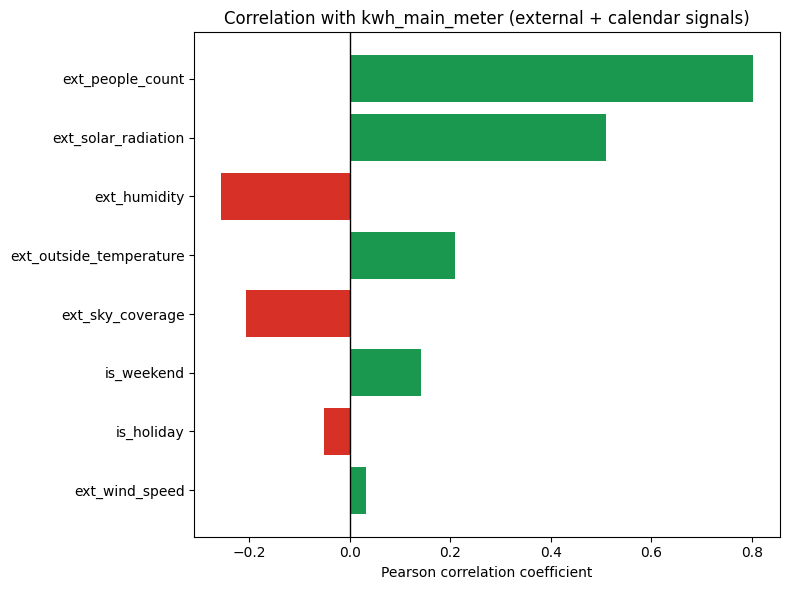
\includegraphics[width=0.9\textwidth]{images/feature-improtance.png}
	\caption{Empirical Pearson correlation of contextual and external drivers with the main electricity meter over the created dataset from \ac{BOPTEST}.}
	\label{fig:feature-importance}
\end{figure}

\section{Data Segmentation and Anomaly Injection}
\label{sec:benchmark-anomalies}

The annual baseline was segmented into multiple training--evaluation regimes to assess sample efficiency and seasonal generalization, including six-month, three-month, and two-week windows. Injected anomalies were constrained to remain below 5\% of total points to preserve realistic anomaly prevalence on the main meter and sub-meters (see Section~\ref{rw:unrealistic-anomaly-ratios}).

Synthetic perturbations emulate realistic operational, control, and contextual fault classes such as sustained drifts, extended deviations, off-hours activity, pattern shifts, and localized spikes. Each anomaly is labeled with onset, duration, and magnitude to support fine-grained evaluation of detection latency, persistence coverage, and financial attribution.

\begin{figure}[htbp]
	\centering
	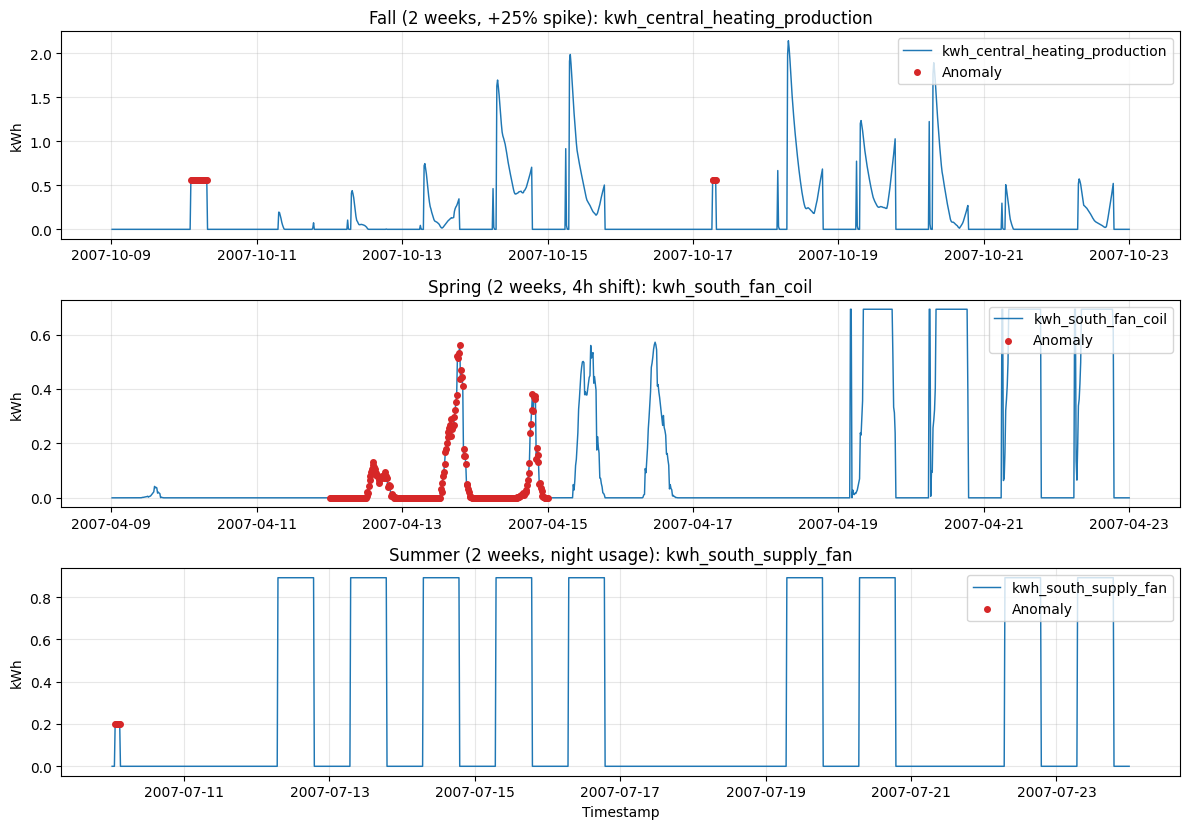
\includegraphics[width=0.92\textwidth]{images/anomaly-dataset-examples.png}
	\caption{Representative sub-meter excerpts from the curated benchmark slices (fall spike, spring pattern shift, summer off-hours). Red markers indicate anomaly windows where the targeted device deviates from its baseline regime.}
	\label{fig:anomaly-dataset-examples}
\end{figure}


\section{Evaluation Constraints and Benchmark Limitations}
\label{sec:benchmark-limitations}

While the BOPTEST-based benchmark enables controlled and reproducible evaluation,
several constraints affect the interpretation and comparability of the resulting
metrics.

\subsection{Training Stability and Coverage Bias}

Several evaluated architectures require extensive per-meter hyperparameter tuning.
\ac{MDN}s in particular exhibit high sensitivity to initialization
and regularization, leading to unstable convergence on subsets of meters.

As a consequence, benchmark coverage differs substantially between methods. Aggregate
scores for unstable models are computed over reduced subsets of meters, introducing
implicit coverage bias. Reported performance therefore reflects both detection accuracy
and training robustness under limited tuning budgets.

\subsection{Comparability Across Model Classes}

Trainable models are trained on season-specific clean baseline windows and are
evaluated on held-out segments drawn from the same baseline regime, into which
synthetic anomalies are injected. Anomaly detection therefore operates relative to a
consistent normative reference distribution.

\ac{TSFM} models, in contrast, cannot be conditioned on the evaluation window
itself. They must infer normative behavior exclusively from preceding historical
context, which may belong to a different seasonal or operational regime. As a result,
detection is performed relative to a shifted baseline distribution rather than the true
local operating regime of the evaluation window. This induces a structural evaluation
asymmetry that becomes most pronounced in short-window and seasonal translation
experiments.

The season-matched three-month baseline configuration provides the closest
approximation of comparable operating conditions. In this configuration, Chronos-2
can condition on the complete baseline history within its maximum context length,
thereby minimizing structural disadvantages relative to trainable models.


\subsection{Interpretation Scope}

Benchmark metrics should therefore be interpreted as indicators of practical
deployability and robustness under realistic engineering constraints rather than as
absolute measures of algorithmic superiority. Emphasis is placed on persistence
tracking, qualitative behavior, and economic interpretability rather than raw
aggregate scores alone.

\section{Comparative Model Performance and Structural Evaluation}
\label{sec:comparative-model-performance}

A total of up to 16{,}979 benchmark runs per model were executed across all dataset
slices. Classical \ac{CNN} baselines adapted from the \ac{TSB-AD} benchmark perform poorly on
building-energy telemetry despite strong multivariate results in generic \ac{TSAD}
benchmarks, confirming that autoregressive input windows destabilize \ac{TSAD}.

A \ac{CNN} Feature-Only architecture that relies solely on exogenous contextual drivers
achieves markedly higher detection scores, indicating that contextual baselines
provide superior normative representations for building-scale telemetry.

Figure~\ref{fig:mdn-dense-cnn-baseline-comparison} summarizes the aggregate comparison across benchmark slices, while Figure~\ref{fig:mdn-dense-cnn-baseline-comparison-mainmeter} isolates the building main meter to highlight the effect of stochastic output modeling under stable training conditions.

\begin{figure}[htbp]
	\centering
	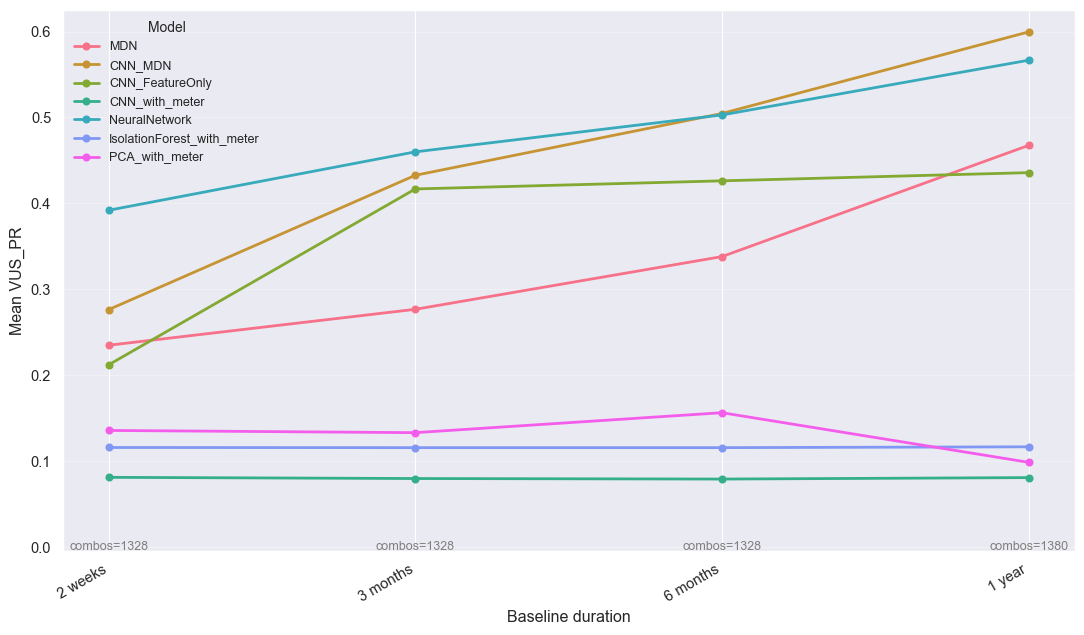
\includegraphics[width=1.0\textwidth]{images/mdn-dense-cnn-baseline-comparison.png}
	\caption{Comparison of neural baselines and mixture-density variants across benchmark slices.}
	\label{fig:mdn-dense-cnn-baseline-comparison}
\end{figure}

\begin{figure}[htbp]
	\centering
	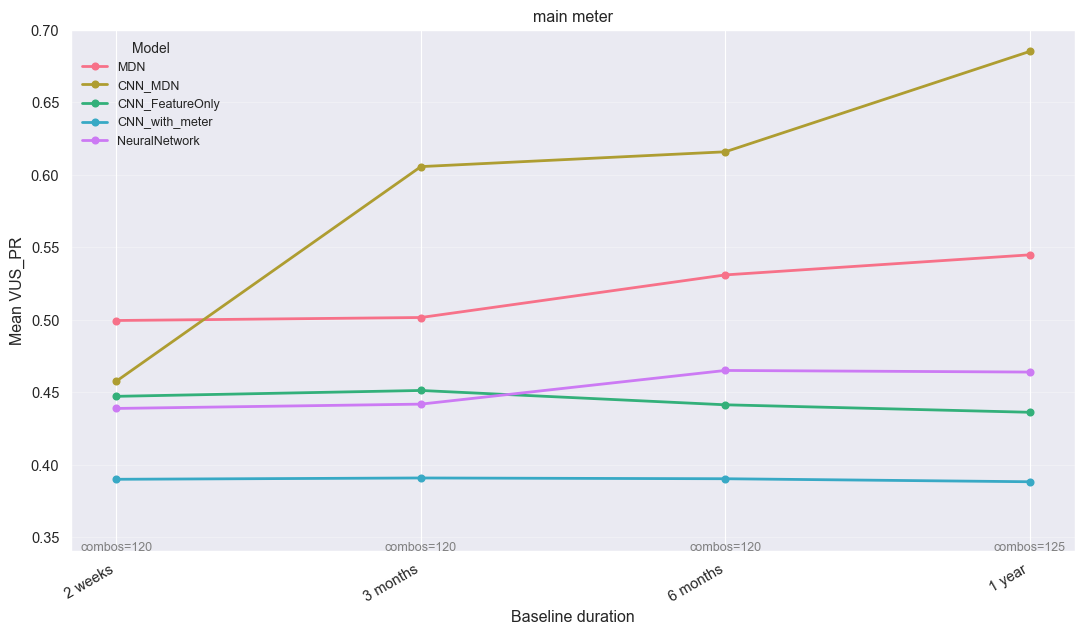
\includegraphics[width=1.0\textwidth]{images/mdn-dense-cnn-baseline-comparison-mainmeter.png}
	\caption{Benchmark comparison on the building main meter, highlighting feature-only and stochastic output effects.}
	\label{fig:mdn-dense-cnn-baseline-comparison-mainmeter}
\end{figure}

\subsection{Stochastic and Hybrid Architectures}
\label{subsec:stochastic-hybrid-architectures}

Pure \ac{MDN}s seem to underperform deterministic contextual models. In
contrast, the hybrid \texttt{CNN\_\allowbreak MDN} delivers the highest \ac{VUS-PR} on
long-horizon baselines, while residual dense networks dominate short-horizon
regimes. Detection accuracy increases monotonically with the amount of baseline
context available for training in almost all models.

\subsection{Training Stability and Classical Baselines}
\label{subsec:training-stability-baselines}

\ac{MDN} layers exhibit sensitivity to initialization and regularization, leading to
coverage gaps across meters. \ac{PCA} and Isolation Forest baselines consistently yield
the lowest performance, confirming that linear and tree-based statistical models fail
to capture the non-linear contextual dependencies present in building-energy
telemetry. The consolidated training history remains available in
Appendix~\ref{app:training-history} (Figure~\ref{fig:training-history-all-meters}).

Importantly, the main meter provides a representative example where \ac{MDN}-based models (including \texttt{CNN\_\allowbreak MDN}) converged stably, which is why Figure~\ref{fig:mdn-dense-cnn-baseline-comparison-mainmeter} is reported separately. In that setting, \ac{MD}-based stochastic output modeling yields a substantially stronger \ac{VUS-PR} than deterministic baselines, suggesting that the weaker aggregate \ac{MDN} scores in Figure~\ref{fig:mdn-dense-cnn-baseline-comparison} are partly a consequence of per-meter instability and reduced coverage rather than an inherent lack of modeling capacity. This limits the strict comparability of aggregated results but still provides evidence for the advantages of probabilistic mixture modeling as discussed in Section~\ref{sec:md-anomaly-scoring}.

\subsection{Season-Matched Three-Month Evaluation}

To minimize seasonal confounding, models were compared under a season-matched
three-month baseline. While \texttt{CNN\_\allowbreak MDN} attains the strongest mean
\ac{VUS-PR}, deterministic neural baselines remain competitive on several anomaly classes.
This configuration is used for the most direct comparison between the foundation model Chronos-2 and trainable baselines, as it minimizes informational asymmetry by aligning the seasonal regime and providing sufficient baseline context.
Chronos-2 performs better than most models, with fine-tuning improving it only minimally in
off-hours detection. PatchTST\parencite{nie2022time} and OmniAnomaly\parencite{su2019robust} underperform, whereas Autoformer\parencite{wu2021autoformer} shows
strong performance on spike-like anomalies.

This comparison is visualized in Figure~\ref{fig:chronos-vs-cnnmdn}.

\begin{figure}[htbp]
	\centering
	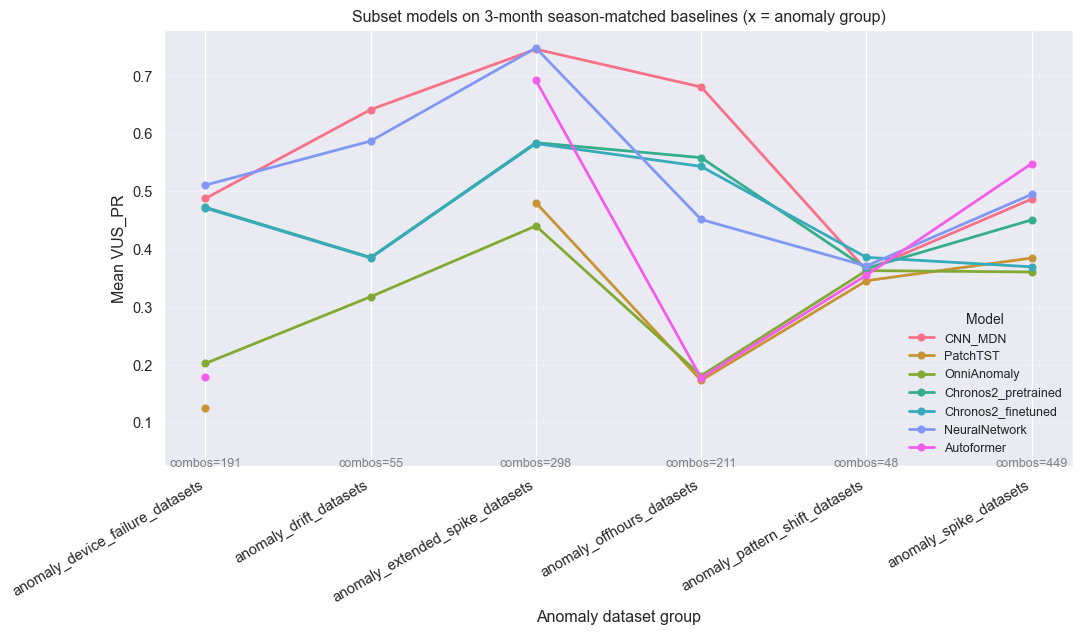
\includegraphics[width=1.0\textwidth]{images/chronos-vs-cnnmdn.png}
	\caption{Chronos-2 vs. \texttt{CNN\_\allowbreak MDN} under season-matched three-month baselines.}
	\label{fig:chronos-vs-cnnmdn}
\end{figure}

\subsection{Seasonal Translation Sensitivity}

Mean \ac{VUS-PR} degrades monotonically as the seasonal distance between training and
evaluation windows increases. The largest performance losses are observed for
\texttt{CNN\_\allowbreak MDN} and OmniAnomaly, while Autoformer and PatchTST remain comparatively
stable across seasonal shifts.

Figure~\ref{fig:seasonal-distance} summarizes this translation sensitivity.

\begin{figure}[htbp]
	\centering
	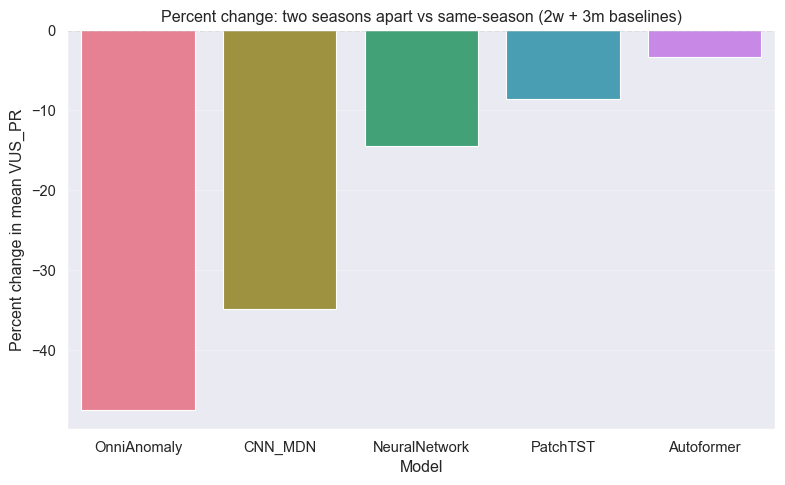
\includegraphics[width=1.0\textwidth]{images/sesonal-distance.png}
	\caption{Seasonal translation sensitivity of mean \ac{VUS-PR} versus seasonal distance.}
	\label{fig:seasonal-distance}
\end{figure}

\subsection{Model Selection Rationale}
\label{sec:model-selection-rationale}

Although \texttt{CNN\_\allowbreak MDN} attains the highest mean \ac{VUS-PR} in most benchmark
configurations, Chronos-2 is selected as the primary deployment model because it best
satisfies the thesis objectives under portfolio-scale constraints. In particular, the
zero-shot, context-conditioned operating mode of \acp{TSFM} directly supports
~\textbf{O\ref{obj:drift-robustness}} by adapting to baseline drift and abrupt
regime changes through recent-context conditioning rather than scheduled per-meter
retraining pipelines. This simultaneously strengthens practical scalability
(~\textbf{O\ref{obj:horizontal-scalability}}) and preserves context-conditioned
normality (~\textbf{O\ref{obj:contextual-fidelity}}).

Trainable baselines require explicit per-meter fitting and repeated retraining to track
non-stationarity, implying fragile orchestration at scale. Persisting anomalies are
prevented from contaminating the adaptive reference by applying Strategy~B from
Section~\ref{sec:inference-time-imputation}, which operationalizes
~\textbf{O\ref{obj:persistence-preservation}} in the deployed pipeline.

While Chronos-2 does not expose an explicit multimodal mixture density, it provides
calibrated, distribution-free quantile bounds (Section~\ref{subsec:quantile-bounds}),
which satisfy ~\textbf{O\ref{obj:distributional-validity}} sufficiently for
deployment. These quantile envelopes enable \ac{QBB} anomaly scoring without
parametric assumptions and avoid the instability and coverage gaps observed for
mixture-density architectures, while remaining competitive in detection accuracy.


\chapter{Implementation}
\label{chap:implementation}

The previous chapter established the methodological framework and the operational requirements for the anomaly detection system. This chapter details the technical realization of these concepts, focusing on the software stack, the integration into the Azure ecosystem, and the internal orchestration logic of the Scala microservice and the Python analytics endpoint.

\section{Integrated System Architecture and Technology Stack}

The implementation utilizes a polyglot approach to leverage the specific strengths of different programming paradigms. While the orchestration and data processing are handled by a Scala microservice to ensure high-performance parallelism, the predictive modeling is realized through a Python endpoint optimized for machine learning.

\subsection{Deployment and Cluster Integration}

The system is designed as a modular Docker container that operates within the same Azure Kubernetes Services (AKS) cluster as the core Eliona microservices. This co-location ensures low-latency communication between the detection logic and the primary data storage. The architecture remains environment-agnostic; for on-premise deployments, the entire stack, including the analytics endpoint, can be executed locally as a suite of interconnected containers.

\begin{figure}[htbp]
	\centering
	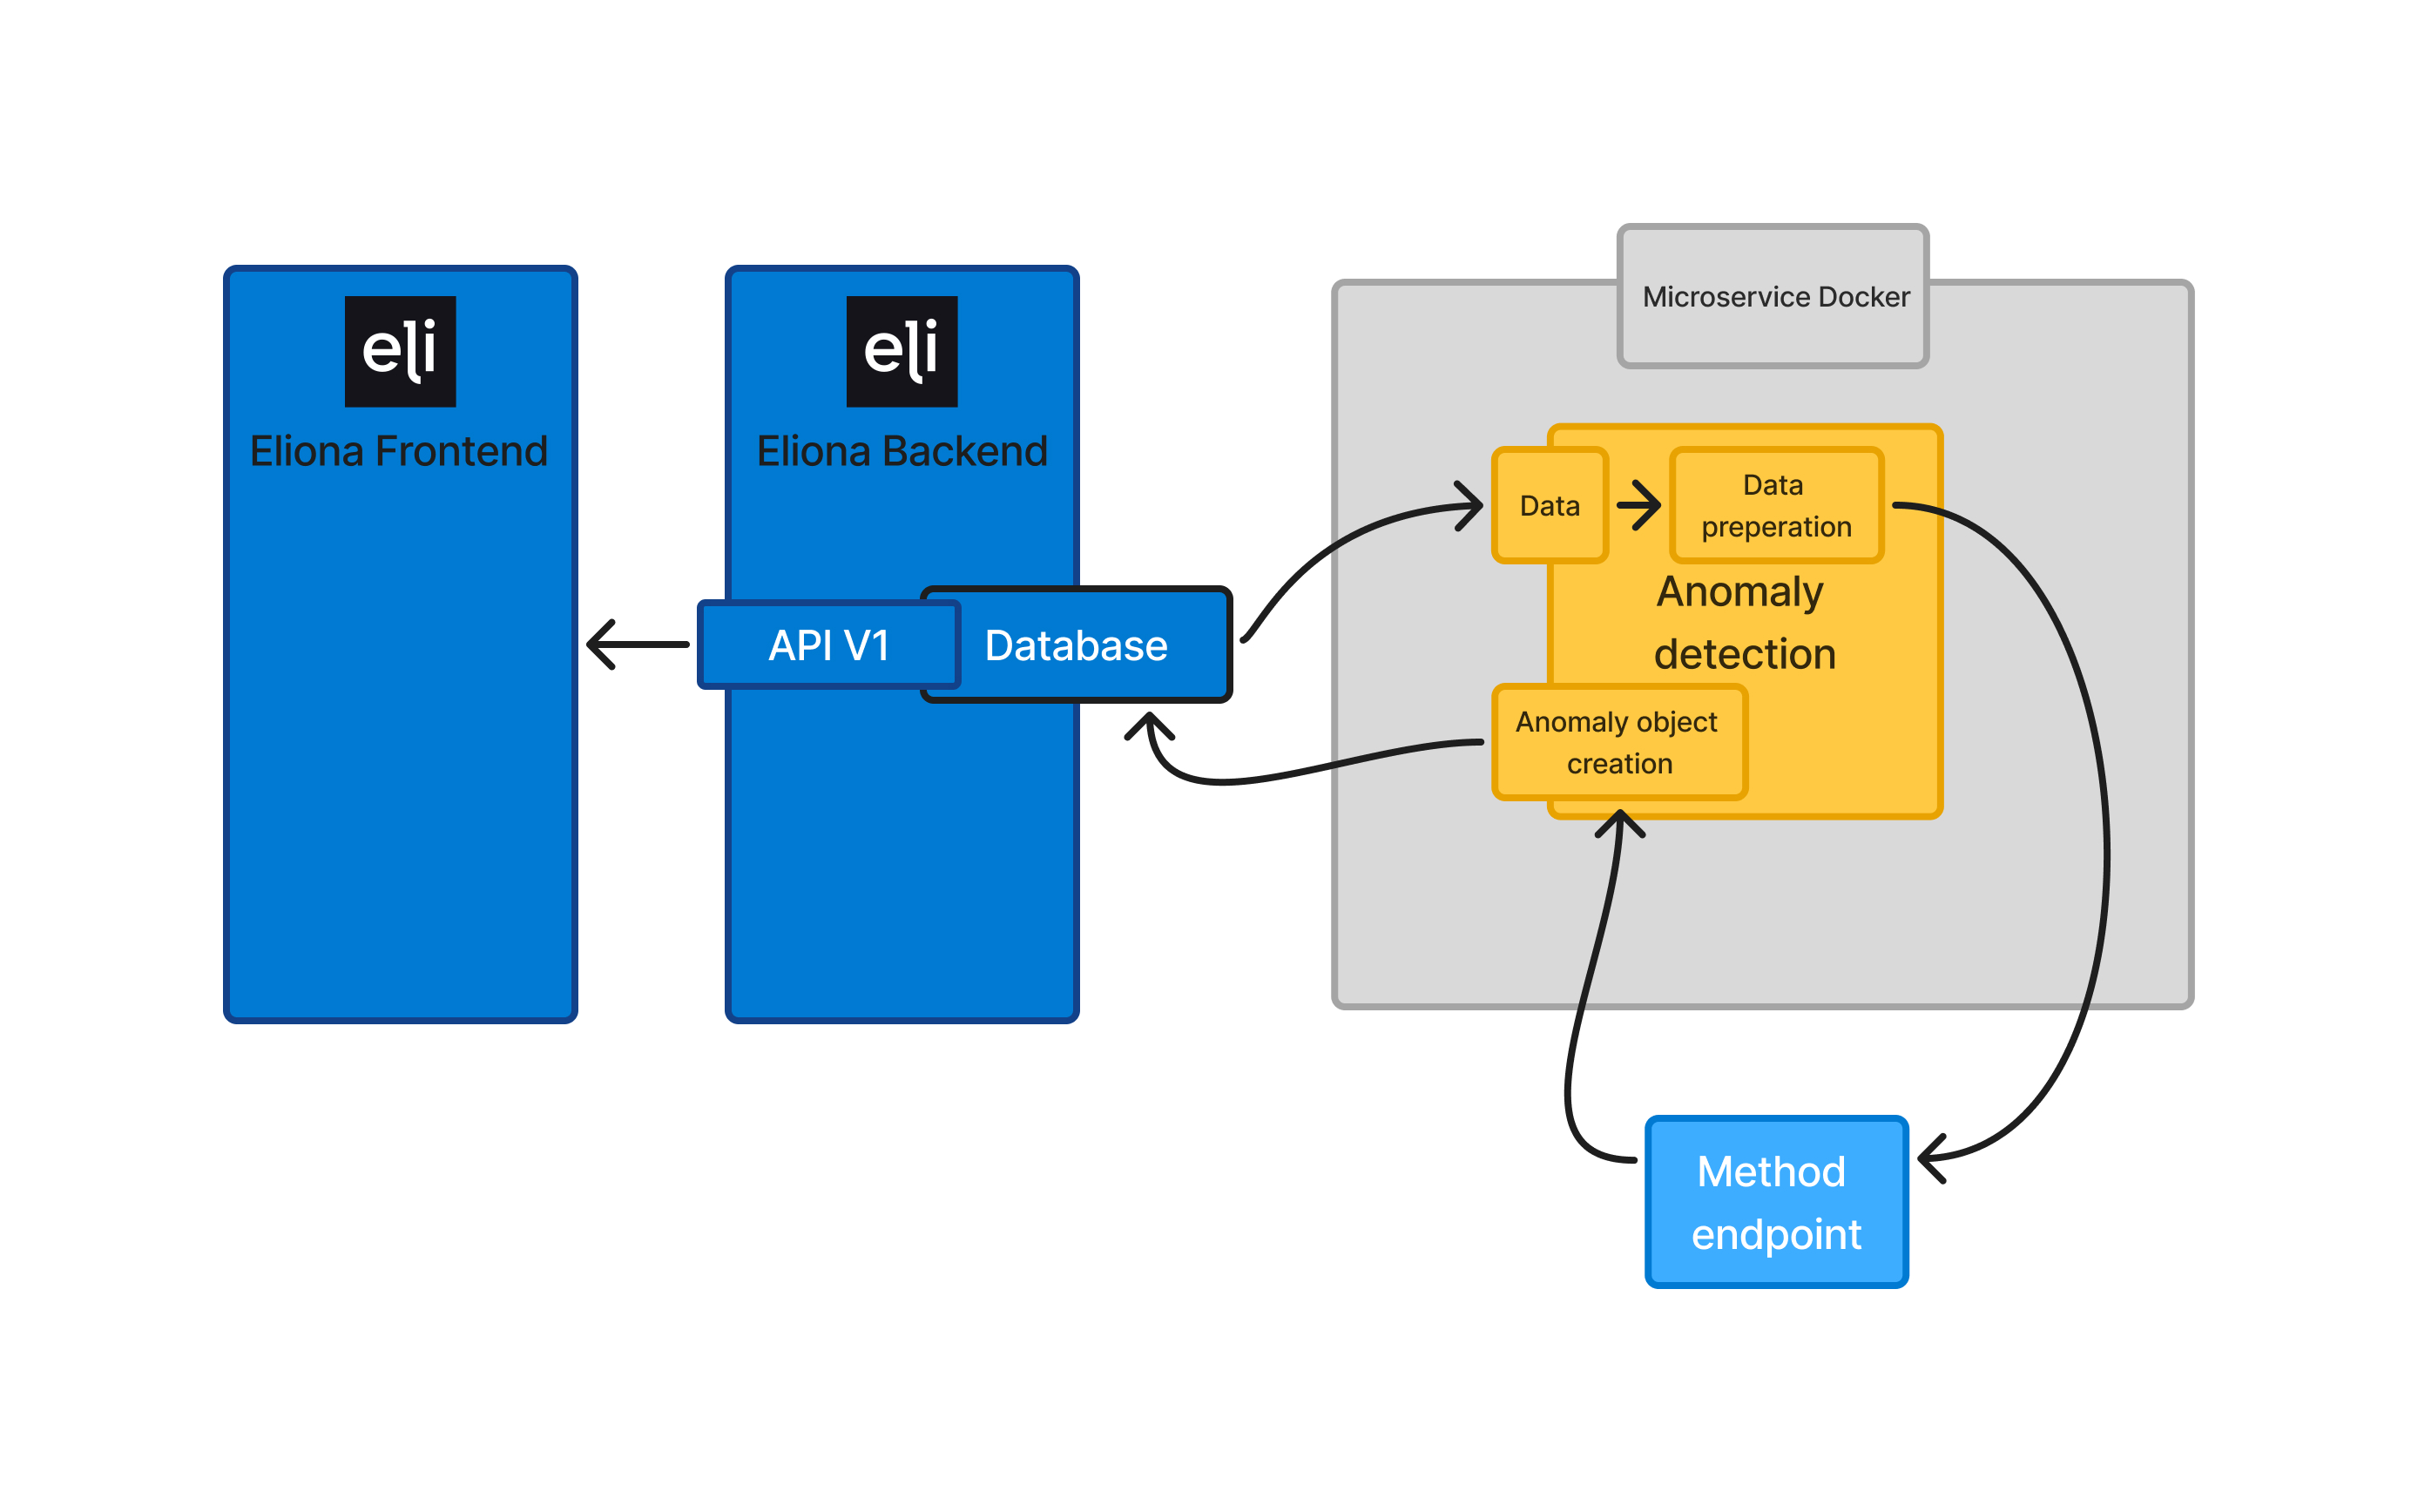
\includegraphics[width=1.0\textwidth]{images/first-high-level-architecture.jpg}
	\caption{High-level deployment of the anomaly detection microservice and Python analytics endpoint within the Eliona and Azure ecosystems.}
	\label{fig:implementation-architecture}
\end{figure}

\subsection{Data Orchestration and Persistence}

The microservice establishes a closed-loop data pipeline with the Eliona backend:

\begin{description}
	\item[Ingestion] Telemetry data is retrieved directly from the centralized PostgreSQL/TimescaleDB instance.
	\item[Analytics loop] After performing data preparation, the microservice transmits multivariate tensors to the method endpoint.
	\item[Synthesis and storage] If the returned predictions indicate a deviation, the service creates an anomaly object. These objects are persisted in the database, where they become accessible to the Eliona frontend via API~V1 for visualization and reporting.
\end{description}

\section{Chronos-2 Analytics Endpoint}

The analytical core is implemented as a dedicated Python microservice hosting the
Chronos-2 transformer model. The service processes batched multivariate time series,
receiving historical context and exogenous covariates and returning probabilistic
quantile forecasts that define the regime-conditioned normative envelope.

For production deployment, the service is exposed as a managed online endpoint in
Azure Machine Learning. This provides automated horizontal scaling, versioned model
management, and containerized deployment, enabling seamless operation in both cloud
and on-premise environments while supporting non-stationary adaptation requirements.

\section{Scala Microservice: Multi-Tenant Orchestration}

System-wide orchestration is implemented as a dedicated Scala microservice that
coordinates data ingestion, contextual enrichment, anomaly scoring, and tenant-level
isolation. Predictive inference is delegated to the Python Chronos-2 endpoint, while
the Scala layer performs all asynchronous I/O, scheduling, and hierarchical
orchestration.

Scala is selected for its strong static typing and high-throughput concurrency model,
enabling safe parallel processing of large multivariate telemetry tensors and complex
building ontologies under multi-tenant operation.

\subsection{Multi-Tenant Lifecycle Management}

Tenants are managed through a centralized orchestration layer that enforces strict
logical isolation across organizations. Independent worker pipelines are instantiated
per tenant and operate on disjoint telemetry scopes, ensuring that ingestion,
processing, and anomaly attribution remain isolated across building portfolios.

Tenant lifecycles are synchronized periodically with licensing and configuration
state. Worker pipelines are automatically instantiated, restarted, or terminated in
response to tenant state changes, ensuring fault tolerance and consistent multi-tenant
operation without manual intervention.

\section{Data Acquisition and Processing Pipeline}

Raw building telemetry is transformed into structured model inputs through a
multi-stage pipeline that performs attribute selection, contextual enrichment, and
robust data conditioning.

\subsection{Attribute Selection and Hierarchical Scoping}

Energy-relevant telemetry channels are identified using semantic attribute metadata
and unit normalization. To ensure operational relevance and computational efficiency,
attributes with negligible economic impact are excluded. Anomaly detection is
performed on the upper hierarchy levels (aggregate and floor meters), while
subordinate assets are retained exclusively for diagnostic attribution.

\subsection{Contextual Enrichment}

External environmental drivers are incorporated via site-localized weather covariates
derived from geographical coordinates. This contextual enrichment enables
disambiguation between technical faults and demand variations induced by weather
conditions.

\subsection{Data Conditioning and Gap Resilience}

Telemetry is aggregated across multiple temporal resolutions and subjected to
gap-resilient conditioning. Transmission gaps and recovery artifacts are corrected
through redistribution mechanisms, while integrity flags preserve explicit data
quality context. Previously detected anomalous values are recursively imputed using
their predicted medians to prevent contamination of subsequent inference windows.

\subsection{Reactive Synchronization}

Model inputs are refreshed on a reactive schedule aligned with finalized aggregation
cycles, ensuring that inference is performed exclusively on complete and consistent
telemetry segments.

\section{Stochastic Inference and Anomaly Quantification}

Anomaly detection is performed by interpreting stochastic quantile forecasts
produced by Chronos-2 under a feature-driven inference strategy.

\subsection{Feature-Driven Inference}

To avoid sequential adaptation effects, inference is conditioned exclusively on
historical context and exogenous covariates (weather, occupancy, temporal indicators),
while the consumption value at the evaluated timestamp is withheld. This enforces
contextual rather than autoregressive normative modeling.

\subsection{Quantile-Based Scoring}

Requests are batched across meters and temporal resolutions. Chronos-2 returns
distribution-free quantile envelopes that define regime-conditioned normative bands.
Extreme quantiles define anomaly boundaries, while central quantiles serve as
conservative economic baselines.

An anomaly is triggered if the observation lies outside the extreme quantile envelope.
Signed deviations are measured relative to the central quantile to quantify waste
or savings under multimodal operating regimes. Deviations below a minimum economic
threshold are discarded to suppress negligible events.

\section{Hierarchical Root Cause Analysis (RCA)}

Upon detection of an aggregate-level anomaly, all subordinate assets in the functional
hierarchy are analyzed to localize the physical origin of the deviation.

\subsection{Diagnostic Attribution}

Sub-meter telemetry is re-evaluated to estimate asset-level financial contributions.
Impacts are attributed both at individual asset level and aggregated by semantic asset
categories (e.g., HVAC, lighting, plug loads), enabling identification of systematic
inefficiencies and dominant fault contributors.

\subsection{Localization and Contextual Enrichment}

Attributed root causes are enriched with spatial metadata and localized environmental
context to support interpretation and remediation planning.

\section{Temporal Collapse and Persistence}

Telemetry is evaluated across multiple temporal resolutions, which may generate
overlapping anomaly events. A temporal collapse mechanism consolidates lower-resolution
detections into higher-resolution events, preventing redundant alerts and preserving
the most conservative financial impact estimate across scales.

\section{AI Synthesis and Action Recommendation}

High-impact anomalies are forwarded to an interpretation layer that synthesizes
localized diagnostics, financial impact, and contextual metadata into structured
human-readable explanations and remediation recommendations using a domain-specialized
large language model (LLM). The LLM operates exclusively at the interpretation layer and
does not influence detection or scoring logic.

\section{Tenant-Specific Configuration}

Detection sensitivity, financial thresholds, and economic parameters are governed by
tenant-specific configuration profiles. These profiles enable adaptation to
organization-specific risk tolerance and energy pricing while preserving strict
multi-tenant isolation and auditability.




\section{Frontend Integration for Operational Decision Support}

The frontend constitutes the operational interface of the anomaly detection framework.
It exposes detected anomalies, quantified financial impact, hierarchical root causes,
and AI-synthesized recommendations in a multi-tenant environment, enabling human
validation and remediation workflows.

\subsection{Centralized Anomaly Registry and Validation Loop}

Detected anomalies are presented in a centralized registry that supports triage,
filtering, and prioritization by financial impact, severity, and affected assets
(Fig.~\ref{fig:anomaly-list}). Human operators can confirm or invalidate anomalies,
forming a controlled human-in-the-loop feedback channel. Invalidated anomalies are
excluded from future baseline construction to prevent contamination of normative
profiles.

\begin{figure}[htbp]
	\centering
	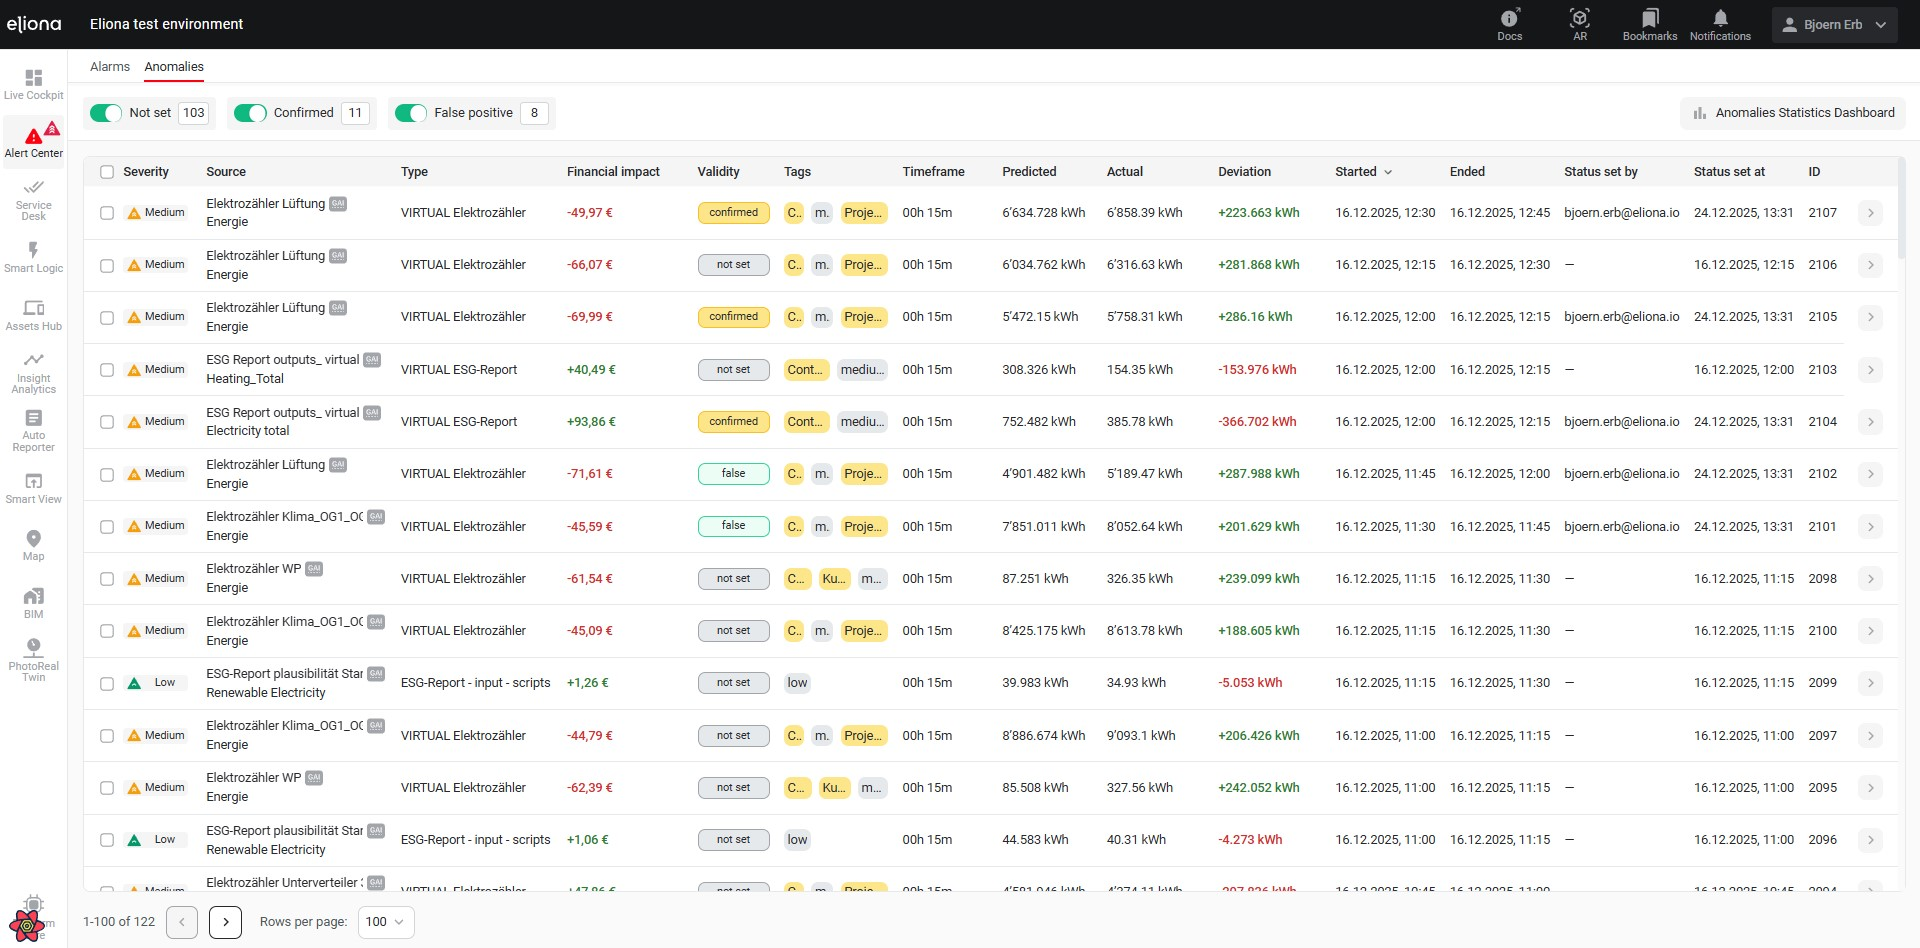
\includegraphics[width=1.0\textwidth]{images/anomaly-list.jpg}
	\caption{Central anomaly registry supporting prioritization, financial impact
	assessment, and validation workflows.}
	\label{fig:anomaly-list}
\end{figure}

\subsection{Quantile Visualization and Diagnostic Context}

Stochastic normative envelopes and anomalous deviations are visualized directly on
consumption charts using quantile-based uncertainty bands (Figs.~\ref{fig:anomalies-in-analytics}
and~\ref{fig:anomaly-analytic-dashboard}). These overlays enable severity assessment
relative to regime-conditioned baselines rather than absolute residual magnitudes.

\begin{figure}[htbp]
	\centering
	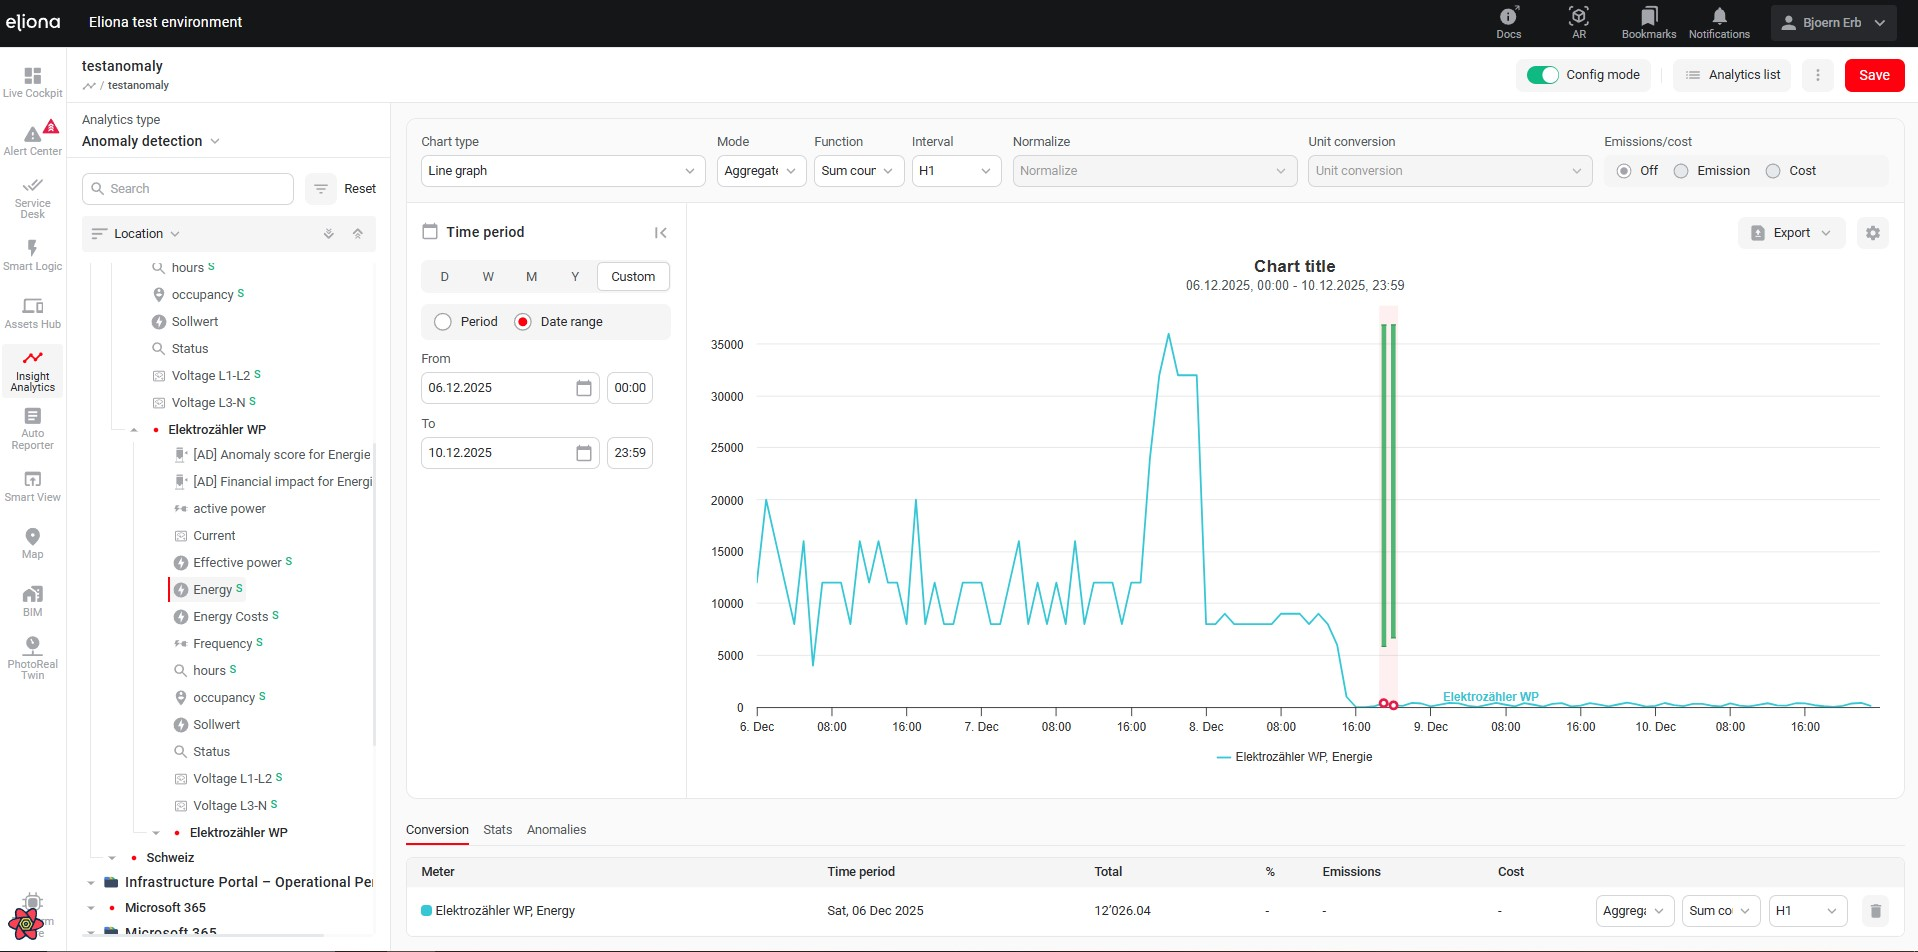
\includegraphics[width=1.0\textwidth]{images/anomalies-in-analytics.jpg}
	\caption{Quantile-based normative envelopes and anomaly overlays within analytics.}
	\label{fig:anomalies-in-analytics}
\end{figure}

\begin{figure}[htbp]
	\centering
	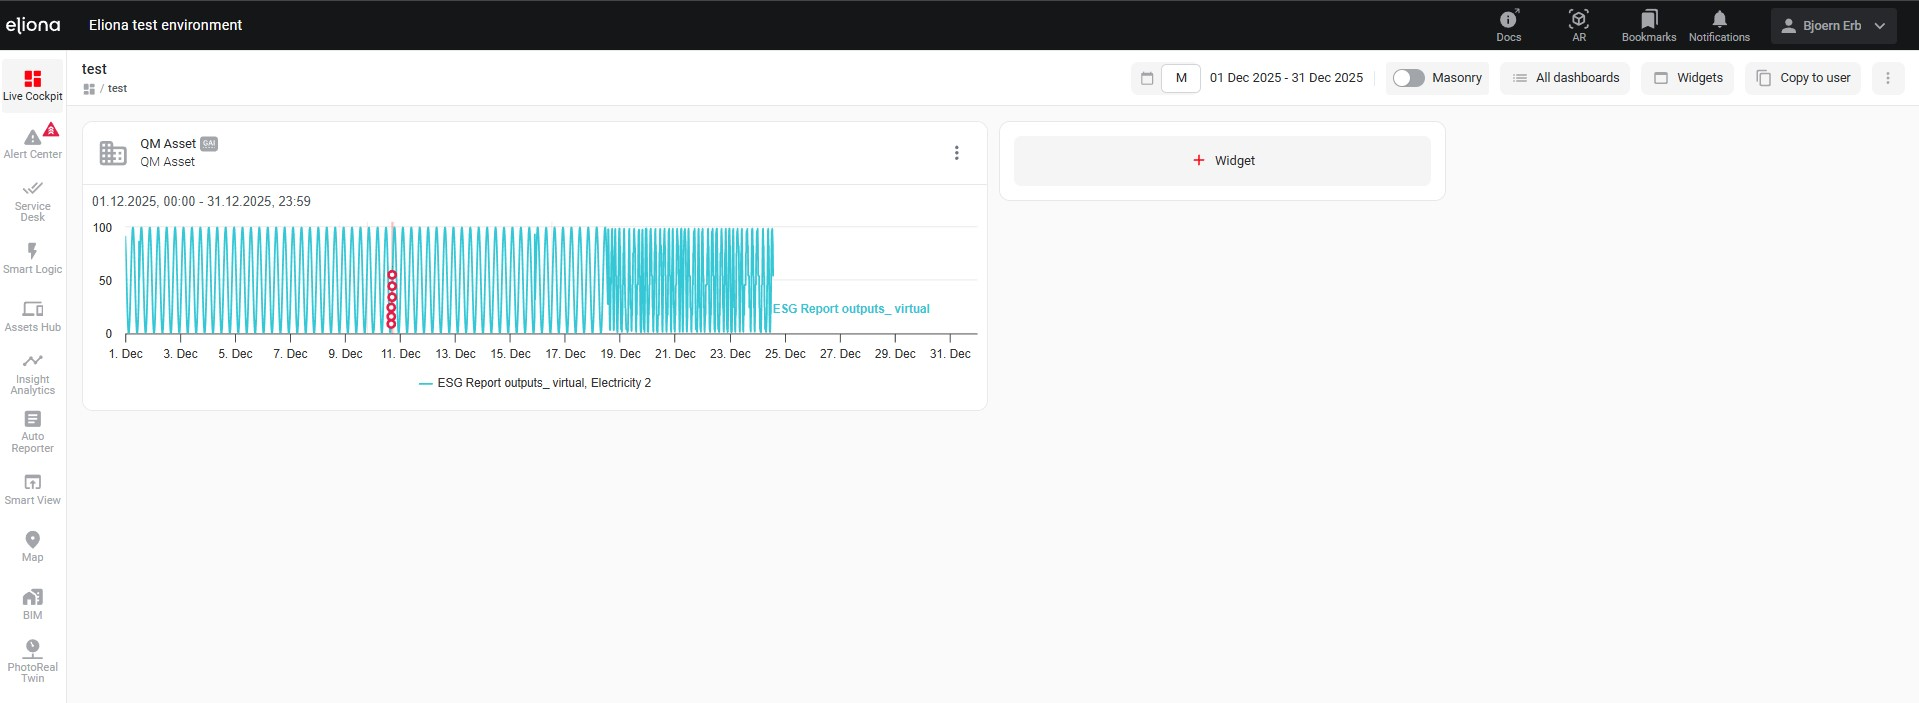
\includegraphics[width=1.0\textwidth]{images/anomaly-analytic-in-dashboard.jpg}
	\caption{Anomaly analytics embedded into operational dashboards.}
	\label{fig:anomaly-analytic-dashboard}
\end{figure}

\subsection{Contextual Tooltips and AI Synthesis}

Interactive tooltips expose localized financial impact, root cause attribution,
validation status, and AI-generated recommendations at individual anomalous points
(Fig.~\ref{fig:anomaly-tooltip}). This supports immediate contextual interpretation.

\begin{figure}[htbp]
	\centering
	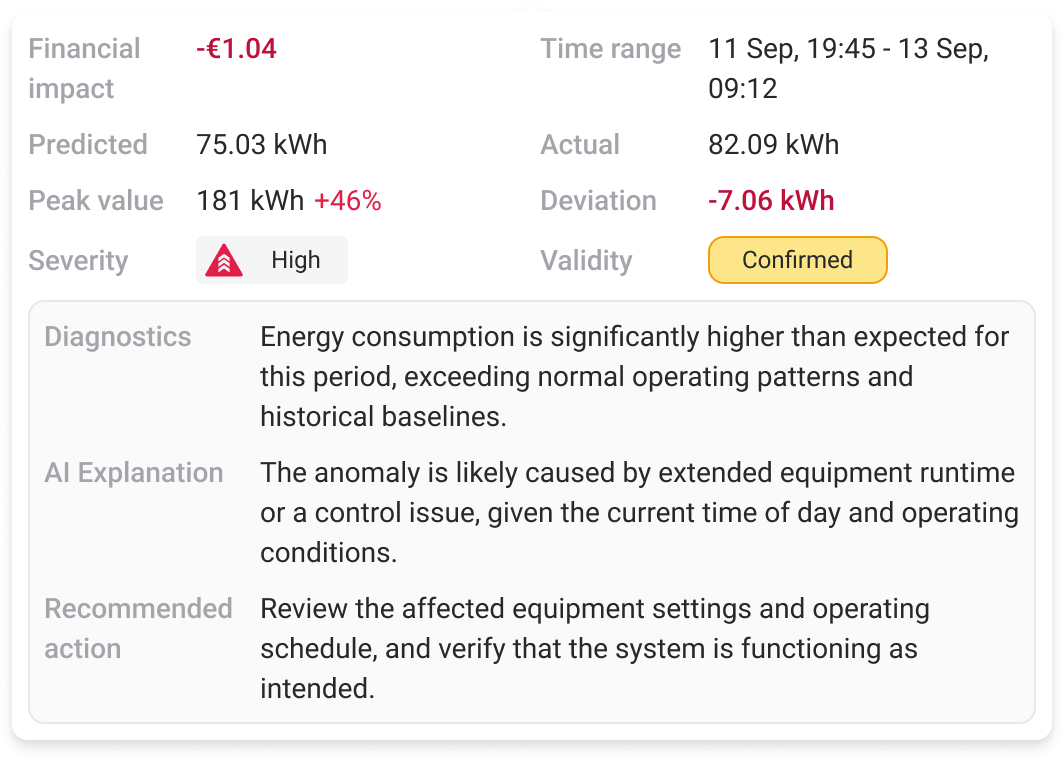
\includegraphics[width=0.8\textwidth]{images/Tooltip.png}
	\caption{Interactive diagnostic tooltip with financial impact and AI synthesis.}
	\label{fig:anomaly-tooltip}
\end{figure}

\subsection{Anomaly Detail View and Action Synthesis}

A dedicated anomaly detail view consolidates quantitative metrics, hierarchical root
causes, contextual metadata, and AI-generated remediation guidance into a single
operational workspace (Fig.~\ref{fig:anomaly-detail-view}), enabling transition from
detection to remediation.

\begin{figure}[htbp]
	\centering
	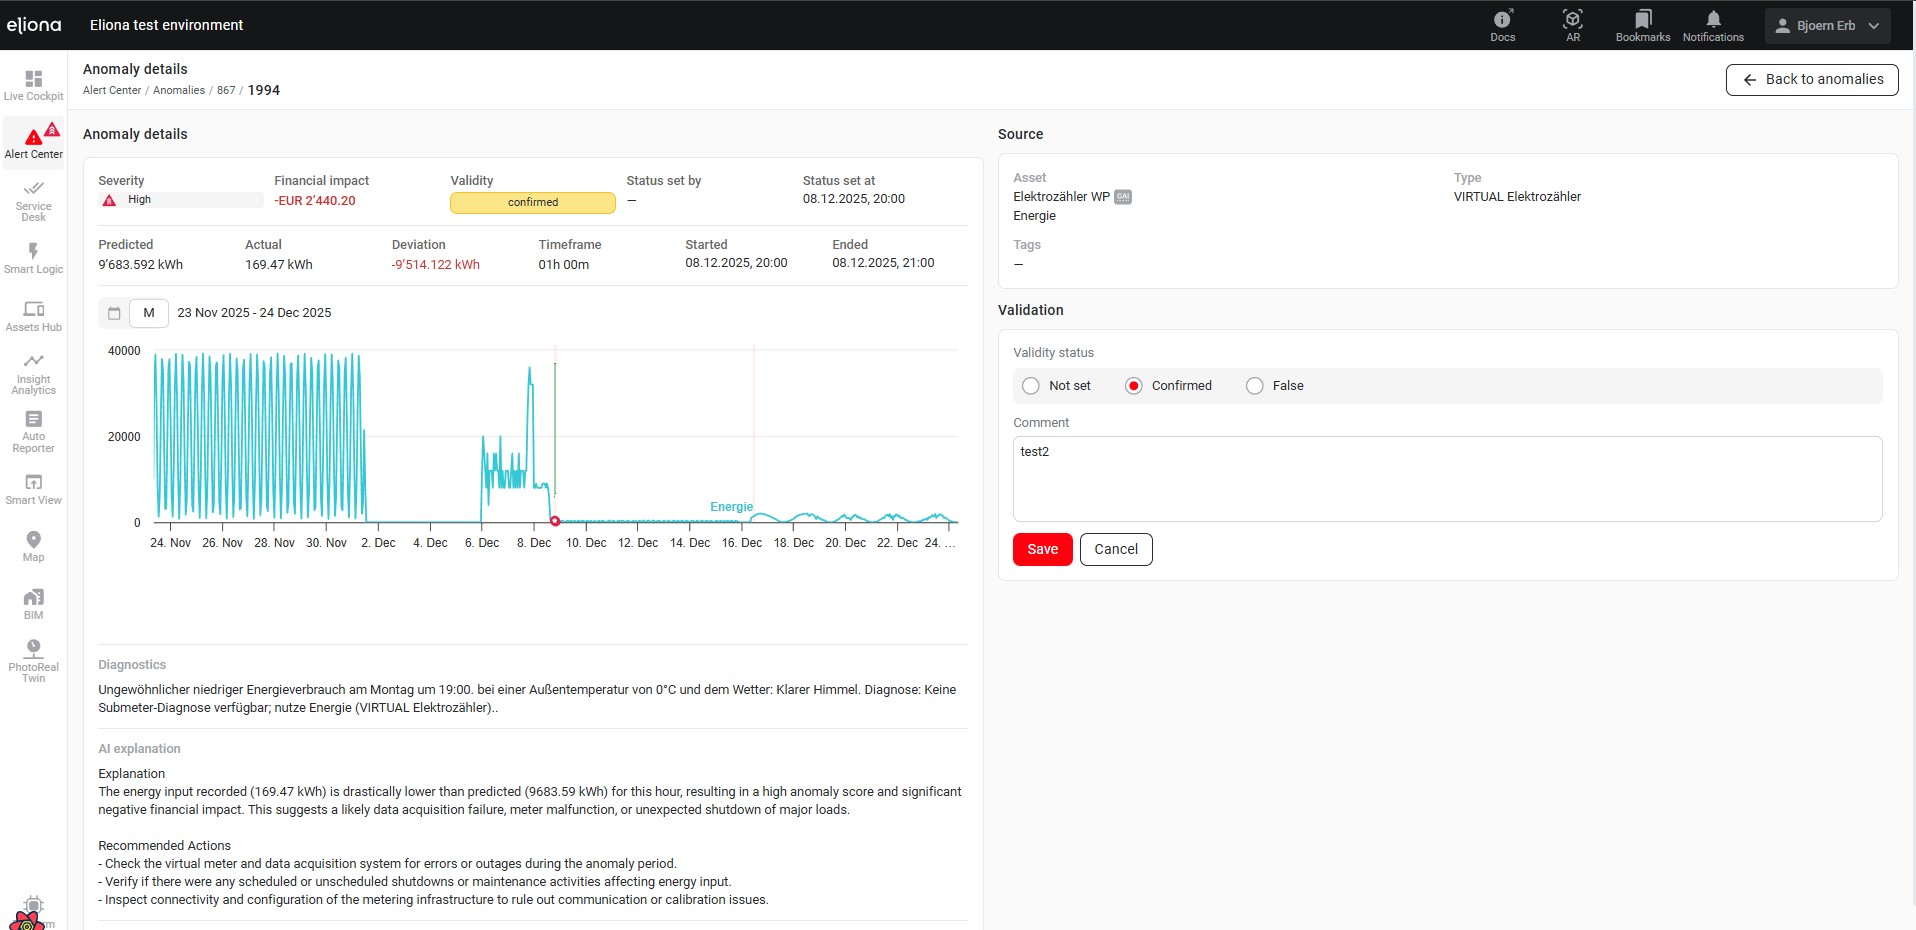
\includegraphics[width=1.0\textwidth]{images/anomaly-details-page.jpg}
	\caption{Integrated anomaly detail view combining financial impact, diagnostics, and
	AI-generated recommendations.}
	\label{fig:anomaly-detail-view}
\end{figure}

\subsection{Macro-Level Reporting and Portfolio Analytics}

Portfolio-level dashboards aggregate anomalies across tenants and sites, providing
executive visibility into financial impact, dominant asset categories, and temporal
patterns (Fig.~\ref{fig:anomaly-statistics-dashboard}). Heatmap visualizations reveal
systematic operational inefficiencies across time-of-day and day-of-week regimes.

\begin{figure}[htbp]
	\centering
	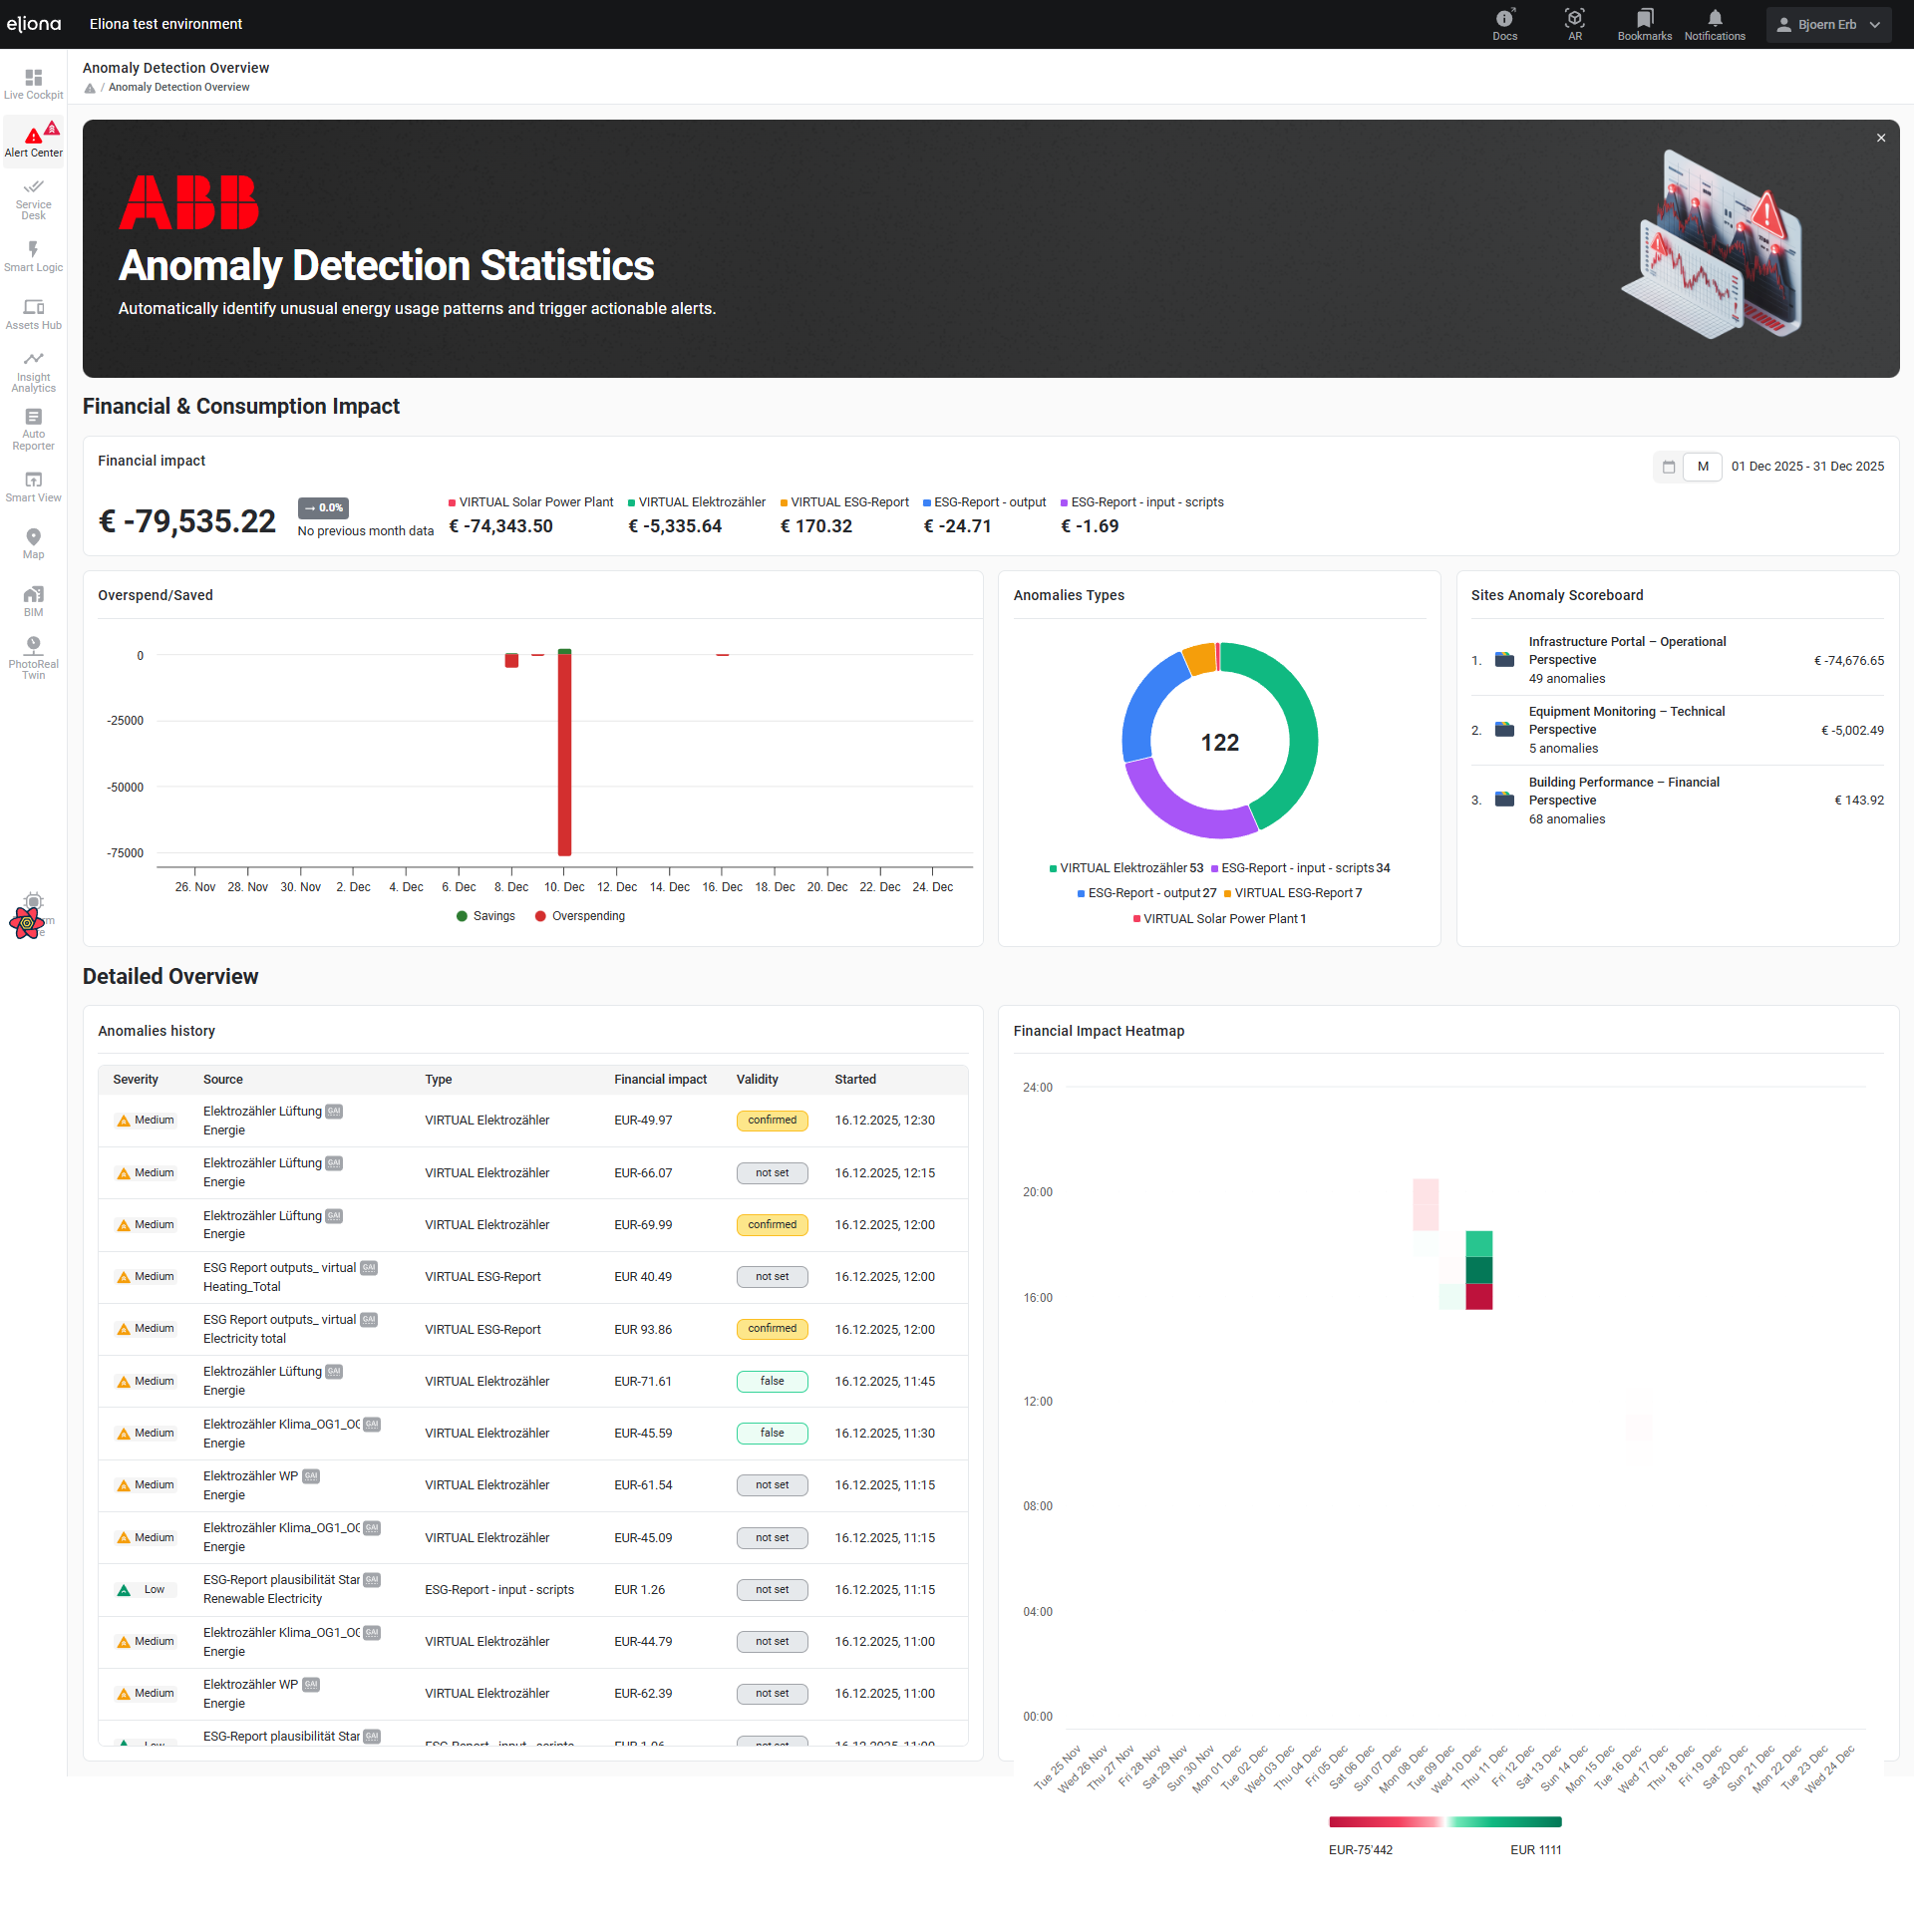
\includegraphics[width=1.0\textwidth]{images/anomalies-statistic-dashboard.png}
	\caption{Portfolio-level anomaly analytics and financial impact aggregation.}
	\label{fig:anomaly-statistics-dashboard}
\end{figure}

\subsection{Asset-Scoped Anomaly Integration}

Anomalies are integrated into asset detail views to support localized diagnostics and
historical inspection of deviations at the equipment and zone level
(Fig.~\ref{fig:anomalies-asset-details}).

\begin{figure}[htbp]
	\centering
	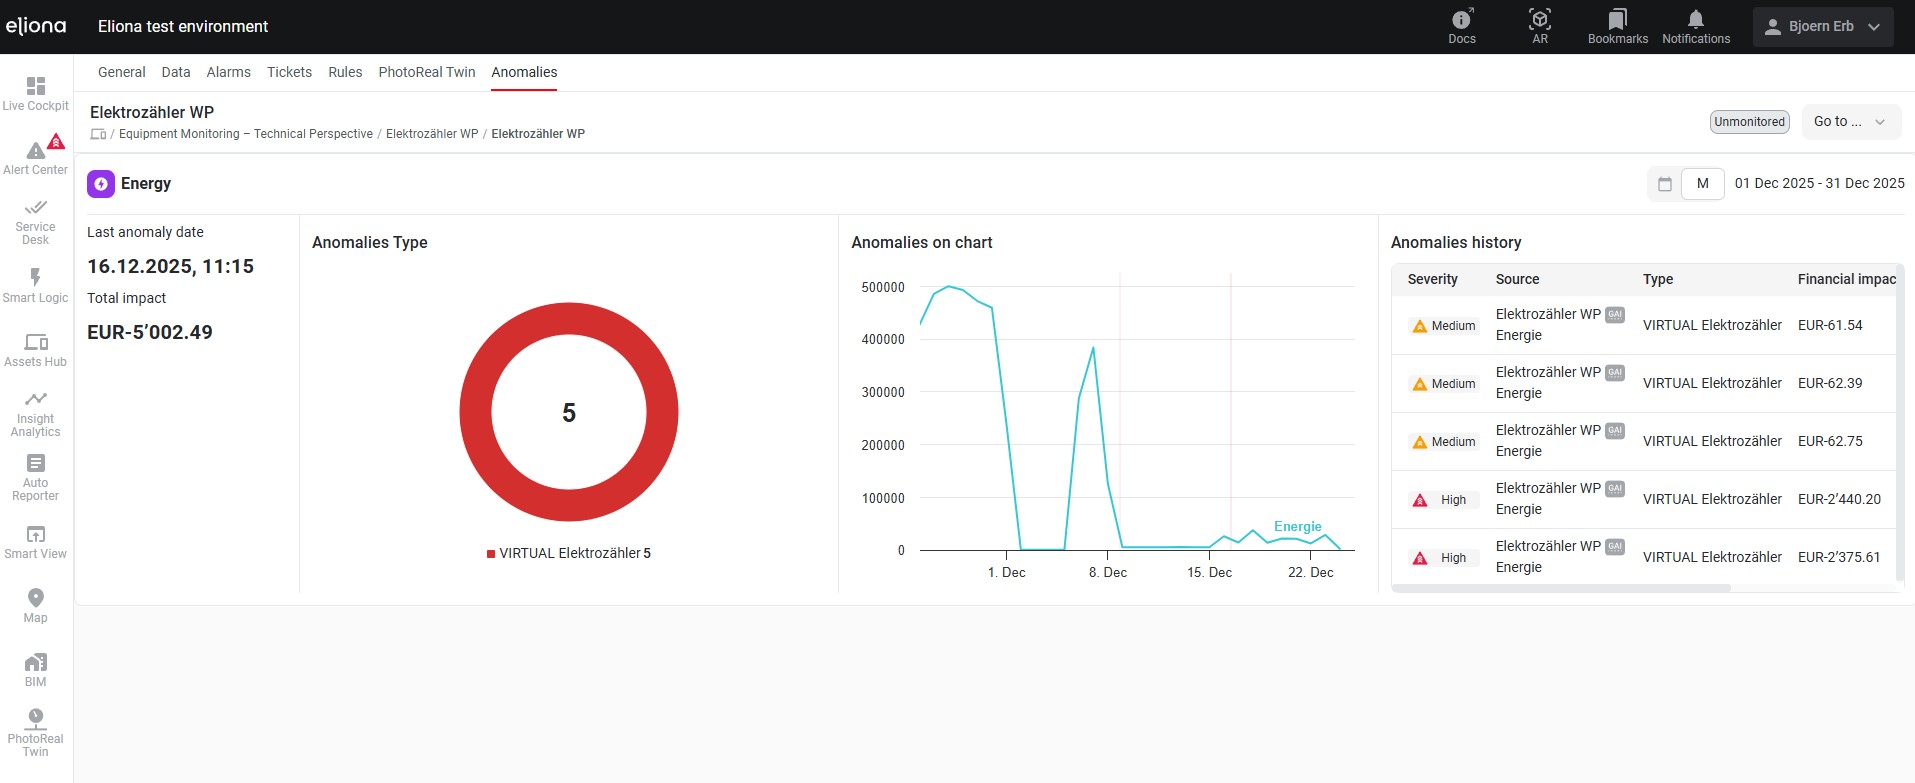
\includegraphics[width=1.0\textwidth]{images/anomalies-in-asset-details.jpg}
	\caption{Asset-level anomaly integration enabling localized inspection and triage.}
	\label{fig:anomalies-asset-details}
\end{figure}

\section{Implementation Summary}
The realized system fulfills the formal design objectives by providing an infinitely
scalable, cloud-native multi-tenant architecture for portfolio-scale building
monitoring. It performs stochastic multivariate anomaly detection using
distribution-free quantile modeling, accurately capturing multimodality and intrinsic
uncertainty in non-stationary energy telemetry.

The system adapts continuously to evolving operational regimes while preventing
persistent anomalies from being absorbed into normative baselines through explicit
human validation mechanisms. Detected deviations are translated into conservative
financial impact estimates, visualized through interpretable uncertainty envelopes,
and localized via hierarchical root cause analysis. A domain-specialized large language
model further synthesizes diagnostic evidence into actionable operational insights,
completing an end-to-end, economically interpretable anomaly management pipeline.

\chapter{Discussion and Future Work}
\label{chap:discussion-future}

The evaluation of the integrated system demonstrates that combining probabilistic
forecasting with hierarchical \ac{RCA} yields actionable, economically interpretable
anomaly management at portfolio scale. At the same time, the transition from a
controlled synthetic benchmark to heterogeneous industrial deployments exposes
limitations in contextual observability, baseline health assumptions, and the
expressiveness of sequential foundation models. This chapter reflects critically on
these gaps and outlines concrete directions for strengthening methodological coverage
and operational robustness.

\section{Critical Reflection on System Design}

The current \ac{RCA} implementation localizes anomalies primarily through signed
financial attribution across sub-meters (Section~\ref{sec:root-cause-analysis}).
This is effective for answering \emph{where} excess consumption accumulates and
supports \textbf{O\ref{obj:hierarchical-diagnosability}} and
\textbf{O\ref{obj:economic-interpretability}}, but it provides limited insight into
\emph{why} the deviation occurred within the control layer
(Foundations Section~\ref{sec:building-energy-data} / causal chain discussion in
Section~\ref{subsec:causal-chain-energy-consumption}). In many facilities, the same consumption pattern can arise
from distinct causes (e.g., manual override, schedule misconfiguration, actuator
fault). Future iterations should therefore extend diagnostics beyond metering
attribution by incorporating \emph{operational state signals} for major consumers
(e.g., valve positions, fan speeds, compressor staging, setpoints). This would enable
causal consistency checks such as: ``is the spike explained by a corresponding change
in control demand?'' and would strengthen context-aware interpretation
(\textbf{O\ref{obj:contextual-fidelity}}) while improving the explainability of
high-impact events.

A second design boundary is the \emph{scope of anomaly classes}. The proposed framework
is strong at detecting deviations in consumption relative to context-conditioned
baselines, but it may not
detect \emph{logic conflicts that are consistently present in the baseline}, such as
simultaneous heating and cooling, chronic simultaneous reheat, or persistent
inefficiencies that have become ``normal'' operation. This is not a modelling failure
but a baseline-definition limitation and directly relates to
\textbf{O\ref{obj:persistence-preservation}}.

\section{Robust Baseline Health Without Manual User Selection}
\label{sec:baseline-health-future}

The current production assumption is that historical data preceding activation is
sufficiently healthy for establishing a normative reference. In real buildings this
is frequently violated: persistent faults may exist for months, and ``normal'' may
already include inefficiency (Foundations Sections~\ref{subsec:temporal-autocorrelation-persistence}
and~\ref{subsec:statistical-distribution-stochastic-noise} on non-stationarity and
persistence; Section~\ref{sec:critique-sequential} on contamination effects). A manual
``gold-standard baseline'' UI would shift responsibility to the operator and does not
scale across tenants, contradicting the deployment objective
\textbf{O\ref{obj:horizontal-scalability}}.

A more robust direction is to integrate \emph{classical rule-based energy baselining
and detection} as a complementary layer, as discussed in
Section~\ref{sec:classical-energy-anomaly-detection}. Rule-based checks (e.g., schedule
violations, simultaneous heating/cooling, minimum runtime constraints, holiday/weekend
rules) can be used in two ways:

\begin{enumerate}
    \item \textbf{Baseline screening:} automatically tag historical intervals as
    ``likely healthy'' vs.\ ``likely faulty'' and preferentially sample healthy
    segments for the model context. This reduces the risk that persistent faults are
    learned as normal and strengthens \textbf{O\ref{obj:persistence-preservation}} and
    \textbf{O\ref{obj:contextual-fidelity}} without requiring user intervention.

    \item \textbf{Coverage expansion:} detect fault classes that are not consumption
    outliers but are operational contradictions (e.g., heating and cooling overlap)
    even if they were present in the baseline. This provides robustness against
    unhealthy historical data and complements the probabilistic deviation detector.
\end{enumerate}

Operationally, this hybrid approach would yield a more complete anomaly portfolio:
probabilistic scoring for contextual deviations (weather/occupancy adjusted) and
deterministic rules for control-logic violations and persistent inefficiencies. The
combination directly addresses the failure mode described in
Section~\ref{sec:critique-sequential} (adaptation and contamination) and improves
diagnostic depth beyond pure metering attribution.

\section{Context and Modality Expansion}

The current implementation focuses on electricity meters enriched with meteorological
covariates. A natural extension is to generalize the same pipeline to additional
utilities (e.g., gas, water, thermal energy, and emissions-related signals), thereby
broadening applicability while preserving the same methodological objectives of
context-conditioned baselines and signed impact quantification
(\textbf{O\ref{obj:contextual-fidelity}}, \textbf{O\ref{obj:economic-interpretability}}).

\section{Future Architecture: Universal Energy Feature Forecaster}
\label{sec:universal-feature-forecaster}

Chronos-2 was selected for deployment due to its operational scalability and robust
quantile outputs (Section~\ref{sec:model-selection-rationale}), but the implementation
also exposes structural limitations of sequential time-series foundation models:

\begin{itemize}
    \item \textbf{Sequence constraint:} inference requires temporally contiguous
    context immediately preceding the forecast timestamp, limiting the ability to use
    non-contiguous ``healthy'' reference segments (Section~\ref{sec:baseline-health-future}).

    \item \textbf{Autoregressive sensitivity:} sequential dependence can amplify
    short-term autocorrelation and induce adaptation effects (Section~\ref{sec:critique-sequential}),
    requiring mitigation logic in production.

    \item \textbf{Limited distribution access:} forecasts are primarily consumed as
    quantile bounds, which enables calibrated envelopes but does not expose an
    explicit multimodal density comparable to \acp{MDN} (Sections~\ref{subsec:mdn-solution}
    and~\ref{sec:md-anomaly-scoring}).
\end{itemize}

A forward-looking direction is a specialized foundation model designed explicitly as a
\emph{universal energy feature forecaster}. Instead of next-step sequence prediction,
the model would perform conditional regression from \emph{context features} to a target
distribution:
\[
p(y \mid \mathbf{x}, \mathcal{B}),
\]
where $\mathbf{x}$ are covariates (weather, calendar, occupancy proxies, operational
state) and $\mathcal{B}$ is an in-context baseline set of feature--target examples.
Critically, $\mathcal{B}$ would not need to be temporally contiguous or adjacent to
the forecast time; it could be composed from automatically screened healthy segments
across the year (Section~\ref{sec:baseline-health-future}). This directly targets
\textbf{O\ref{obj:contextual-fidelity}}, \textbf{O\ref{obj:drift-robustness}}, and
\textbf{O\ref{obj:persistence-preservation}} by decoupling the normative reference
from immediate sequential inputs.

\subsection{Mixture-Distribution Output and Distribution-Aware Scoring}

To recover the expressiveness of mixture modelling without per-meter training, the
model should output an explicit multimodal density (e.g., token-mixture or continuous
mixture parameters). This would enable likelihood-based and \ac{DQ}-based anomaly
scoring (Section~\ref{sec:md-anomaly-scoring}) with time-comparable severity scaling,
while keeping the zero-shot generalization benefits emphasized in
Section~\ref{sec:model-selection-rationale}. In effect, this would combine the
portfolio robustness of \acp{TSFM} with the distributional fidelity of \acp{MDN},
strengthening \textbf{O\ref{obj:distributional-validity}} without the instability and
coverage gaps observed in trainable mixture architectures.

\subsection{Decision Support and IPMVP-Style Verification}

A feature-conditional, baseline-set forecaster also enables systematic baseline
comparison without retraining: the same operating point (same covariates $\mathbf{x}$)
can be evaluated under multiple baseline contexts $\mathcal{B}_1,\mathcal{B}_2$ to
quantify the expected change attributable to interventions. This naturally aligns with
Measurement and Verification practices such as the \ac{IPMVP}: predicted counterfactual consumption
under a pre-intervention baseline can be compared against a post-intervention baseline
to estimate savings under matched conditions. This extends the system beyond fault
detection into continuous efficiency verification, directly reinforcing the economic
motivation of Chapter~\ref{chap:introduction} and strengthening
\textbf{O\ref{obj:economic-interpretability}} at portfolio scale.
Figure~\ref{fig:ipmvp-overview} summarizes the \ac{IPMVP} comparison workflow that underpins
these verification steps~\parencite{ipmvp-protocol}.

\begin{figure}[H]
\centering
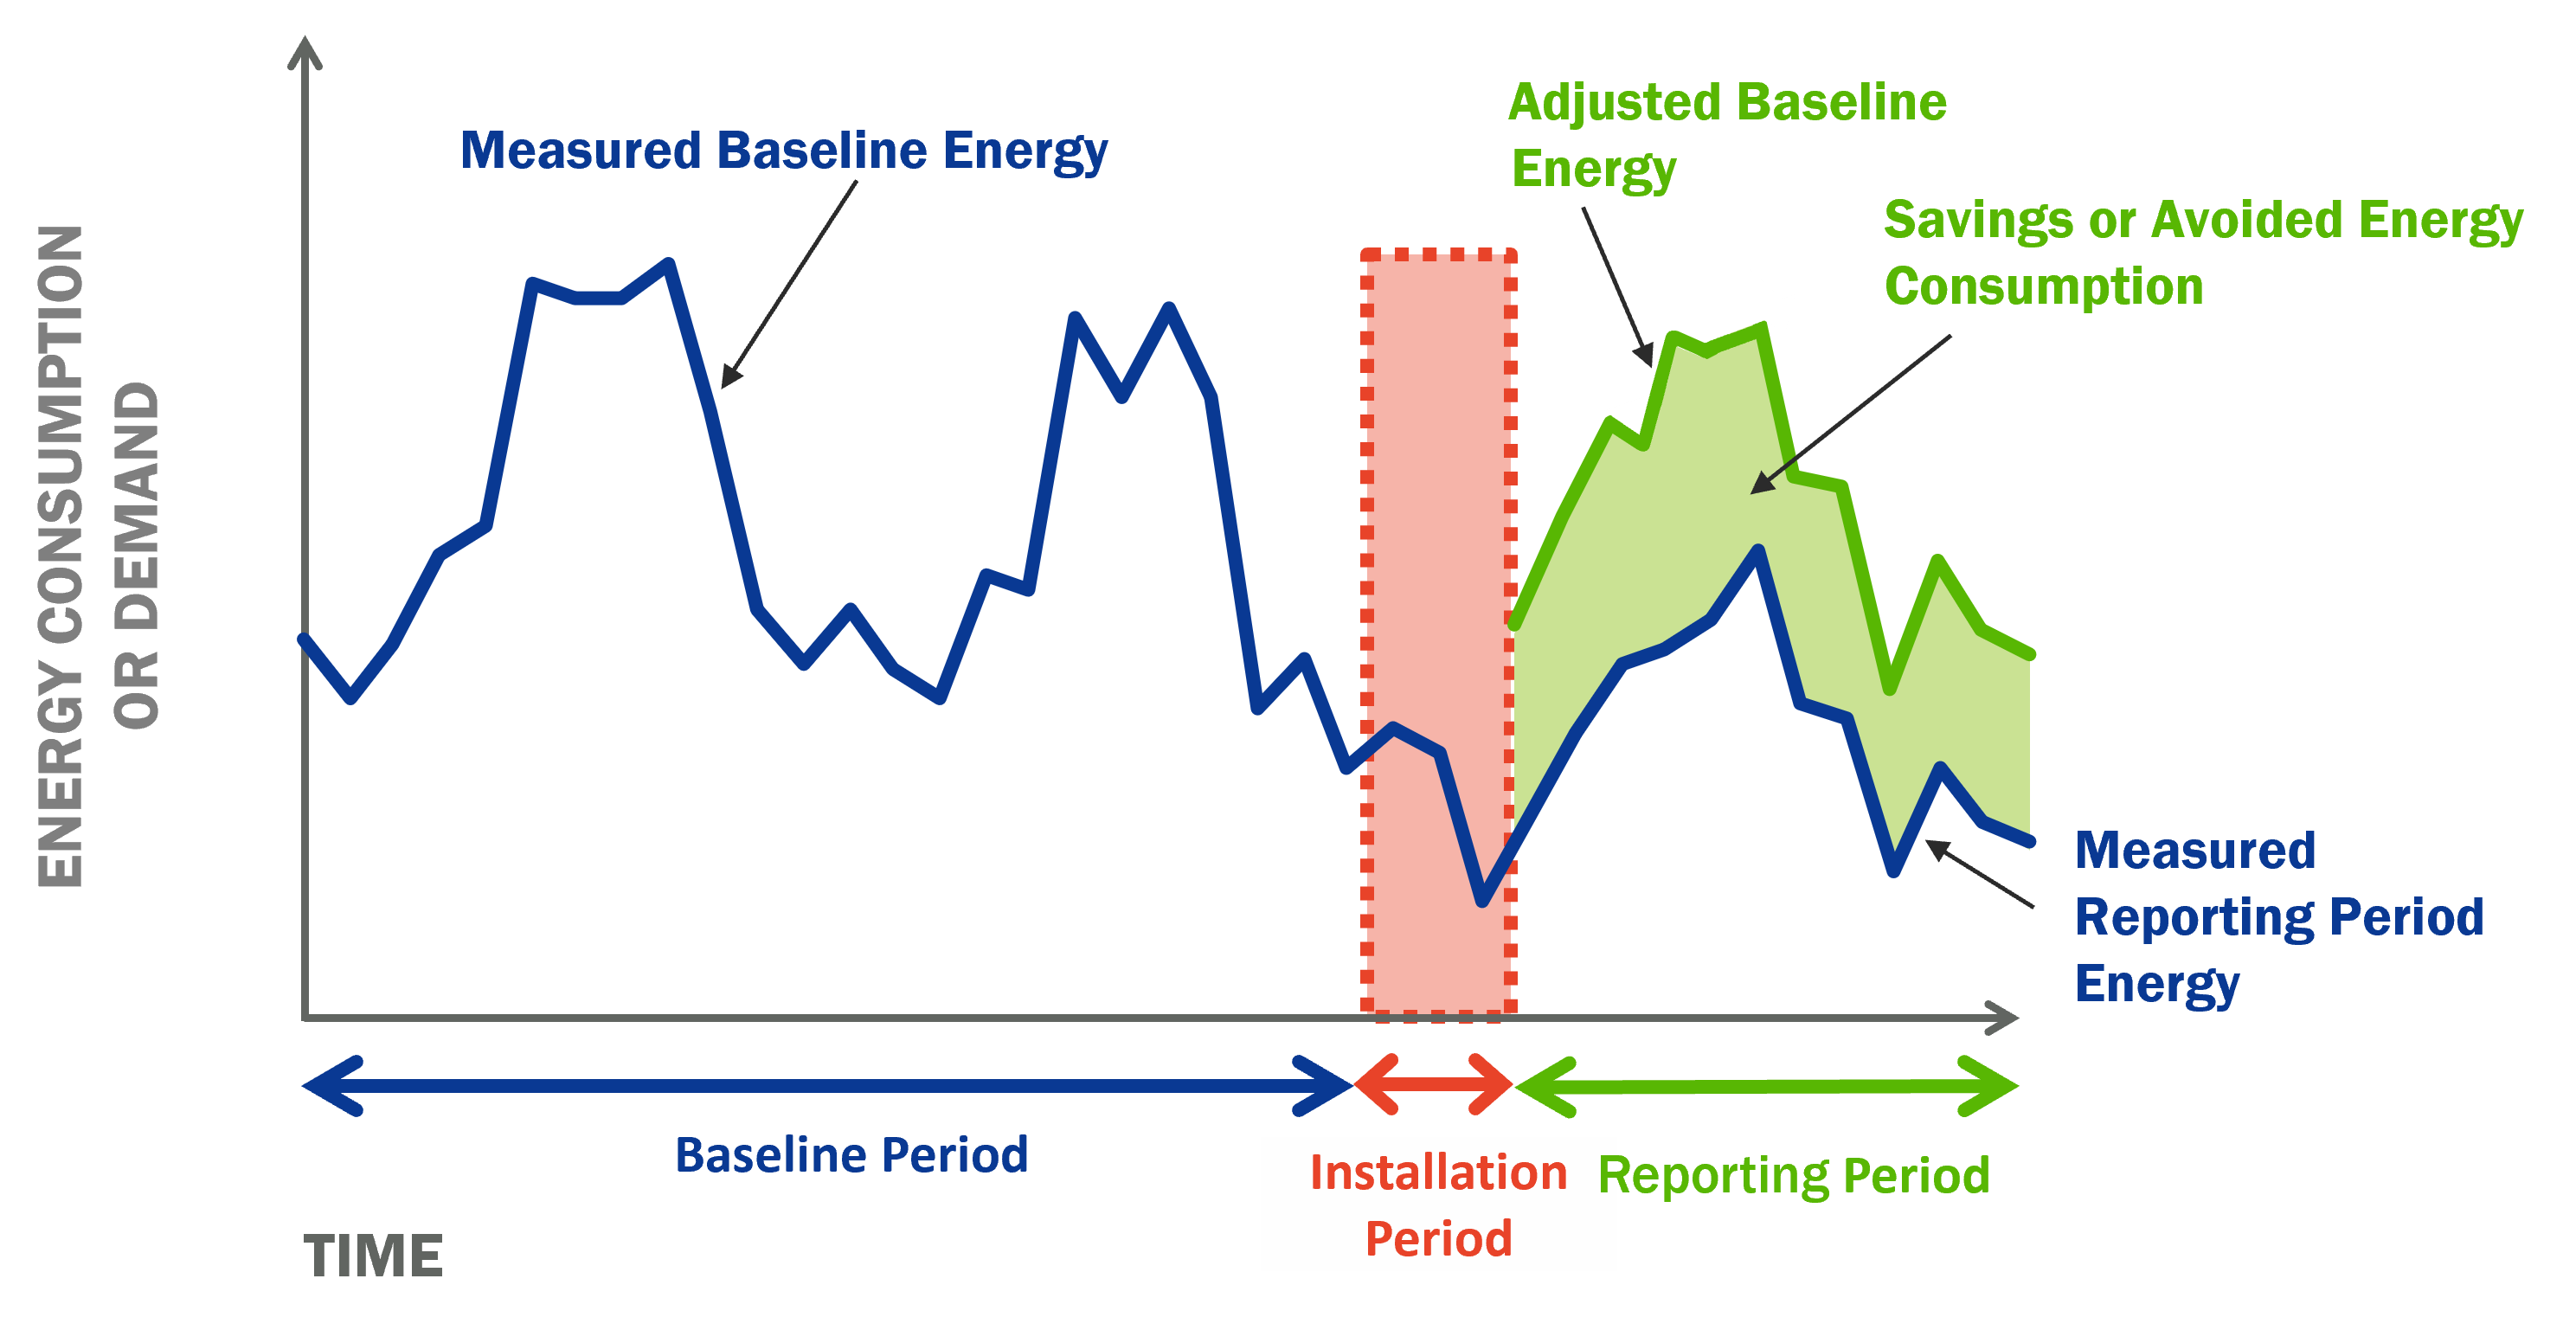
\includegraphics[width=0.85\textwidth]{images/IPMVP.png}
\caption{\ac{IPMVP} verification workflow across baseline and reporting periods, adapted from \textcite{ipmvp-protocol}.}
\label{fig:ipmvp-overview}
\end{figure}


\chapter{Conclusion}\label{chap:conclusion}
This thesis investigated how portfolio-scale building-energy anomaly detection can be
made both operationally deployable and economically actionable. Departing from
threshold-based monitoring and deterministic residual detectors (Section~\ref{sec:critique-sequential}),
the problem was formulated as \ac{MCAD} under multimodality and non-stationarity
(Foundations Sections~\ref{subsec:dimensionality-normality-modes}
and~\ref{subsec:statistical-distribution-stochastic-noise}), with the explicit requirement
that detected deviations be (i) probabilistically well-defined, (ii) monetarily
quantifiable, and (iii) diagnostically localizable within building hierarchies
(Sections~\ref{sec:md-anomaly-scoring},~\ref{sec:financial-impact}, and~\ref{sec:root-cause-analysis}).

Methodologically, the work showed why sequential autoregressive detectors are
structurally brittle for sustained building faults: anomalous values contaminate
sliding windows, error propagates, and long anomalies can be adapted away
(Section~\ref{sec:critique-sequential}). These failure modes motivate
context-conditioned baselines and distribution-aware scoring that remain meaningful
across regime changes (Sections~\ref{sec:inference-time-imputation}
and~\ref{sec:md-anomaly-scoring}).
To support scientific comparison under building-relevant anomaly semantics, a
domain-specific benchmark was constructed using \ac{BOPTEST}, providing labeled,
contextual fault scenarios with seasonal segmentation and realistic anomaly
prevalence (Sections~\ref{sec:benchmark-design} and~\ref{sec:benchmark-anomalies}).

Empirically, the benchmark results reinforced a central design claim: in building
energy telemetry, contextual drivers can be more reliable than autoregressive
history for establishing normative behavior (Section~\ref{sec:comparative-model-performance}).
Classical \ac{CNN} baselines with autoregressive windows performed poorly despite their
strong performance in generic multivariate benchmarks, whereas a feature-only \ac{CNN}
relying on exogenous context achieved markedly higher detection scores
(Section~\ref{sec:comparative-model-performance}). Across up to 16{,}979 runs per model,
the hybrid \texttt{CNN\_\allowbreak{}MDN}~achieved the highest mean \ac{VUS-PR}~under stable
long-horizon training (Section~\ref{subsec:stochastic-hybrid-architectures}), while
mixture-density components exhibited non-trivial initialization and coverage sensitivity
across meters (Section~\ref{subsec:training-stability-baselines}), highlighting the
practical importance of robustness under limited tuning budgets.

On the deployment axis, the thesis delivered a production-grade implementation inside
the Eliona platform (Chapter~\ref{chap:implementation}): a containerized Scala
orchestration service and a Python forecasting endpoint integrated in a multi-tenant
environment with strict tenant scoping, telemetry integrity handling, conservative
signed impact quantification, and hierarchy-aware root cause attribution
(Sections~\ref{sec:financial-impact} and~\ref{sec:root-cause-analysis}). The diagnostic
outputs are surfaced through role-aware workflows (alert triage, analytic overlays,
drill-down detail views) and are complemented by an \ac{LLM} layer restricted to
post-hoc semantic synthesis, preserving traceability by keeping detection and scoring
deterministic (Section~\ref{sec:root-cause-analysis}).

Taken together, the results support three main conclusions. First, building-energy
anomaly detection should be treated as a contextual and distributional modelling
problem rather than a point-residual thresholding task, because multimodal regimes
and non-stationarity dominate real operations (Foundations Section~\ref{sec:building-energy-data}
and Section~\ref{sec:md-anomaly-scoring}). Second, portfolio-scale value requires
economic interpretability and localization (Sections~\ref{sec:financial-impact}
and~\ref{sec:root-cause-analysis}): without signed impact and hierarchical attribution,
detection signals remain difficult to operationalize in maintenance and optimization
workflows. Third, evaluation must reflect persistence and contextuality
(Sections~\ref{sec:critique-sequential} and~\ref{sec:systemic-benchmarking-challenges});
otherwise, reported improvements risk being benchmark artifacts rather than deployable
capability.

Finally, the work clarifies where future progress is most impactful. Hybridizing the
probabilistic detector with complementary rule-based checks, as established in
classical energy monitoring, is a direct path to stronger baseline-health robustness
and broader fault-class coverage (Section~\ref{sec:classical-energy-anomaly-detection}
and Section~\ref{sec:baseline-health-future}). Beyond this, a compelling research
direction is a universal energy feature forecaster that removes the sequence-contiguity
constraint of current time-series foundation models and exposes explicit multimodal
densities for distribution-aware anomaly scoring—while enabling standardized baseline
comparison aligned with measurement and verification practice (e.g., \ac{IPMVP})
\parencite{ipmvp-protocol} (Section~\ref{sec:universal-feature-forecaster}).
%% Use letters for the chapter numbers of the appendices.
\appendix

\input{appendix-a}

\printbibliography[heading=bibintoc]

\end{document}

